%%%%%%%%%%%%%%%%%%%%%%%%%%%%%%%%%%%%%%%%%%%%%%%%%%%%%%%%%%%%%%%%%%%%%%%%%%%%%%%%
% Preámbulo                                                                    %
%%%%%%%%%%%%%%%%%%%%%%%%%%%%%%%%%%%%%%%%%%%%%%%%%%%%%%%%%%%%%%%%%%%%%%%%%%%%%%%%

\documentclass[11pt,a4paper,titlepage,oneside]{report}

%%% RELACIÓN DE VARIABLES A PERSONALIZAR %%%
\def\lingua{gal}
%\def\lingua{esp} % descomenta esta liña se redactarás a memoria en español
%\def\lingua{eng} % descomenta esta liña se redactarás a memoria en inglés
\def\nome{Mateo Amado Ares}                             % substitúe aquí o teu nome
\def\nomedirectorA{José Rouco Maseda}              % substitúe aquí o nome de quen dirixe
\def\nomedirectorB{Jorge Novo Buján}             % duplica esta liña máis veces se o precisas, cambiando
                                                     % a letra final (A, B, C, D...): úsanse na portada.tex
\def\titulo{Aliñamento de imaxes oftalmolóxicas usando representacións neuronais implícitas} % substitúe aquí o título do teu TFG
%\def\titulacion{gced}                               % descomenta esta liña e comenta a seguinte se es estudante do GCED
\def\titulacion{gei}
\def\mencion{COMPUTACIÓN}                           % descomenta a mención que che corresponda se es estudante do GEI
%\def\mencion{ENXEÑARÍA DO SOFTWARE}
%\def\mencion{ENXEÑARÍA DE COMPUTADORES}
%\def\mencion{SISTEMAS DE INFORMACIÓN}
%\def\mencion{TECNOLOXÍAS DA INFORMACIÓN}

%\def\renomearcadros{si} % descomenta esta liña se redactas a memoria en español e prefires que
                         % os "cuadros" e o "índice de cuadros" se renomeen
                         % a "tablas" e "índice de tablas" respectivamente

\usepackage{estilo_tfg}

% Lista de paquetes potencialmente interesantes (uso baixo demanda)

% \usepackage{alltt}       % proporciona o entorno alltt, semellante a verbatim pero que respecta comandos
% \usepackage{enumitem}    % permite personalizar os entornos de lista
% \usepackage{eurofont}    % proporciona o comando \euro
% \usepackage{float}       % permite máis opcións para controlar obxectos flotantes (táboas, figuras)
% \usepackage{hhline}      % permite personalizar as liñas horizontais en arrays e táboas
  \usepackage{longtable}   % permite construir táboas que ocupan máis dunha páxina
% \usepackage{lscape}      % permite colocar partes do documento en orientación apaisada
% \usepackage{moreverb}    % permite personalizar o entorno verbatim
  \usepackage{multirow}    % permite crear celdas que ocupan varias filas da mesma táboa
% \usepackage{pdfpages}    % permite insertar ficheiros en PDF no documento
% \usepackage{rotating}    % permite diferentes tipos de rotacións para figuras e táboas
% \usepackage{subcaption}  % permite a inclusión de varias subfiguras nunha figura
% \usepackage{tabu}        % permite táboas flexibles
% \usepackage{tabularx}    % permite táboas con columnas de anchura determinada

%%%%%%%%%%%%%%%%%%%%%%%%%%%%%%%%%%%%%%%%%%%%%%%%%%%%%%%%%%%%%%%%%%%%%%%%%%%%%%%%
% Corpo                                                                        %
%%%%%%%%%%%%%%%%%%%%%%%%%%%%%%%%%%%%%%%%%%%%%%%%%%%%%%%%%%%%%%%%%%%%%%%%%%%%%%%%

\begin{document}

 %%%%%%%%%%%%%%%%%%%%%%%%%%%%%%%%%%%%%%%%
 % Preliminares do documento            %
 %%%%%%%%%%%%%%%%%%%%%%%%%%%%%%%%%%%%%%%%

 \begin{titlepage}
  
  \hspace*{128pt}
  \textcolor{udcpink}{{\fontencoding{T1}\fontfamily{phv}\selectfont Facultade de Informática}}\\[-32pt]

  \begin{center}
    
\includegraphics[scale=0.3]{imaxes/udc}\\[25pt]

    {\large TRABALLO FIN DE GRAO \\
            \nometitulacion \\
            \nomemencion } \\[10pt]

    \carimbo \\[25pt]

    \begin{huge}
      \begin{spacing}{1.3}
        \bfseries \titulo
      \end{spacing}
    \end{huge}
  \end{center}
  
  \vfill
  
  \begin{flushright}
    {\large
    \begin{tabular}{ll}
      {\bf Estudante:} & \nome \\
      {\bf Dirección:} & \nomedirectorA \\
                       & \nomedirectorB \\ % duplica esta liña máis veces se o precisas, cambiando
                                           % a letra final (A, B, C, D...); define eses nomes no memoria_tfg.tex
    \end{tabular}}
  \end{flushright}
  \rightline{A Coruña, \datasimple.}
\end{titlepage}

 \dedicatoria{Dedicatoria} % escribe neste comando o teu texto de dedicatoria
 \paxinaenbranco
 \begin{agradecementos}
 \blindtext                % substitúe este comando polo teu texto de agradecementos
 \end{agradecementos}
 %%%%%%%%%%%%%%%%%%%%%%%%%%%%%%%%%%%%%%%%%%%%%%%%%%%%%%%%%%%%%%%%%%%%%%%%%%%%%%%%

\pagestyle{empty}
\begin{abstract}
O aliñamento da imaxe oftalmolóxica é un campo moi relevante. Aliñar imaxes médicas é útil para,
entre outras cousas, revisar o avance dunha enfermidade ao longo do tempo. O caso dos ollos é de particular importancia xa que permiten a observación in-vivo de tecido neuronal e vasos sanguíneos. Aliñar as imaxes manualmente é un proceso tedioso e complexo, polo que automatizar este proceso é moi beneficioso.

Neste traballo explórase o uso de redes de representación implícita,
 onde se parametriza a imaxe como unha función continua coas coordenadas como entrada e o valor do pixel como saída, como unha alternativa para o aliñamento de imaxes.
 Estas aportan vantaxes frente a representacións tradicionais discretas como a independencia de resolución e poder prescindir de grandes bases de datos xa que se adestran mediante un proceso de optimización para cada par de imaxes.
 Ademais, en lugar de usar funcións de activación estándar como RELU, adoitan empregar unha función de activación sinusoidal (SIREN), que pode axudar a eliminar o sesgo cara sinais de baixa frecuencia e mapear mellor deformación pequenas e detalladas.

Adaptando o traballo realizado por \cite{wolterink2021implicit}, valoraráse se este método é apto para a tarefa de aliñamento de imaxes oftalmolóxicas e como se compara con métodos convencionais.

  \vspace*{25pt}
  \begin{segundoresumo}
    Ophthalmic image alignment is a highly relevant field. Aligning medical images is useful for, among other things, reviewing the progression of a disease over time. The case of eyes is particularly important as they allow in-vivo observation of neuronal tissue and blood vessels. Manually aligning images is a tedious and complex process, so automating this process is beneficial.
    
    This work explores the use of implicit representation networks, where the image is parameterized as a continuous function with coordinates as input and pixel value as output. This provides advantages over traditional discrete representations such as resolution independence and the ability to dispense with large databases since they are trained through an optimization process for each group of images.
    Furthermore, instead of using standard activation functions like RELU, they typically employ a sinusoidal activation function (SIREN), which can help eliminate bias towards low-frequency signals and better map small and detailed deformations.
    
    Based on the work done by \cite{wolterink2021implicit}, this study will evaluate whether this method is suitable for the task of aligning ophthalmic images and how it compares to conventional methods.
  \end{segundoresumo}
\vspace*{25pt}
\begin{multicols}{2}
  \begin{description}
  \item [\palabraschaveprincipal:] \mbox{} \\[-20pt]
  \begin{itemize}
      \item Imagen médica
      \item Imagen oftalmológica
      \item Aprendizaje profundo
      \item Registro de Imágenes 
      \item Representaciones neuronales implícitas
  \end{itemize}
  
  \end{description}
  \begin{description}
  \item [\palabraschavesecundaria:] \mbox{} \\[-20pt]
  \begin{itemize}
      \item Medical imaging
      \item Ophthalmological imaging
      \item Deep learning
      \item Image Registration
      \item Implicit neural representations (INRs)
  \end{itemize}
  \end{description}
  \end{multicols}
\end{abstract}
\pagestyle{fancy}

%%%%%%%%%%%%%%%%%%%%%%%%%%%%%%%%%%%%%%%%%%%%%%%%%%%%%%%%%%%%%%%%%%%%%%%%%%%%%%%%


 \pagenumbering{roman}
 \setcounter{page}{1}
 \bstctlcite{IEEEexample:BSTcontrol}

 \tableofcontents
 \listoffigures
 \listoftables
 \clearpage
 
 \pagenumbering{arabic}
 \setcounter{page}{1}

 %%%%%%%%%%%%%%%%%%%%%%%%%%%%%%%%%%%%%%%%
 % Capítulos                            %
 %%%%%%%%%%%%%%%%%%%%%%%%%%%%%%%%%%%%%%%%

 \chapter{Introdución}
\label{chap:introducion}

\lettrine{N} este primer capítulo expóñense as motivacións e obxetivos deste traballo. Ademais, detallarase a estrutura da memoria e os apartados que a conforman.

\section{Motivación}
\label{sec:motivacion}

A oftalmoloxía válese da análise de imaxes obtidas por diversos métodos para realizar diagnósticos e seguimentos precisos.
Non obstante, dado que estas imaxes poden prover de distintas modalidades e foron tomadas dende distintos puntos ou en instantes separados no tempo, é preciso aliñalas para poder comparalas de xeito efectivo.
O aliñamento de imaxes é un proceso que se leva a cabo para poder comparar imaxes dun mesmo paciente tomadas en distintos momentos, ou para comparar imaxes de diferentes pacientes.
Consiste en deformar dúas ou máis imaxes de forma que as características de interese se atopen na mesma posición (superpostas).
Este é un proceso tedioso e propenso a erros, polo que calquer mellora nel é de gran interese para os profesionais da saúde. 
Esta tarefa é axeitada para ser automatizada, xa que é non require dun xuízo clínico, senón que se basea na comparación de características visuais das imaxes. A automatización deste proceso permitiría aos profesionais da saúde dedicar máis tempo a tarefas máis relevantes.

Xa existen diversas técnicas para realizar aliñamento de imaxes automático, especialmente ca chegada do deep learning á visión por computador para imaxes médicas, onde unha aproximación habitual é o uso de redes neuronais convolucionais \cite{medicalimageanalysis}.
Estos métodos, aínda que efectivos, teñen limitacións. Unha delas é que requiren dunha gran cantidade de datos para o seu adestramento, o que pode ser un problema en campos como a medicina, onde a obtención de datos é cara e complexa. Ademais, xeralmente teñen unha precisión menor ca métodos automáticos convencionais, pese a que si que son máis rápidos \cite{bharati2022deeplearningmedicalimage}.
Adaptando o traballo realizado por \cite{wolterink2021implicit}, preténdese aplicar redes de representación implícita para o aliñamento de imaxes oftalmolóxicas.

\section{Obxectivos}

Neste traballo explorarase o uso de redes de representación implícita para o aliñamento de imaxes oftalmolóxicas, para determinar se son aptas para esta tarefa e se poden superar as limitacións dos métodos anteriores.
Para iso, os obxectivos específicos son:
\begin{itemize}
    \item Adaptar o traballo de IDIR \cite{wolterink2021implicit} para aplicalo a imaxes oftalmolóxicas.
    \item Comparar o rendemento do método proposto co de métodos automáticos convencionais nos datasets de FIRE \cite{FIRE} e RFMID \cite{RFMiD}.
    \item Analizar a influencia de distintos parámetros no rendemento do método proposto, en particular a influencia da función de activación SIREN.
\end{itemize}

\section{Estructura }

Nesta sección detallarase a estrutura da memoria e os apartados que a conforman.

\begin{itemize}
    \item \textbf{Capítulo 1: Introdución}: neste capítulo introdúcese o traballo, explicando as motivacións e obxetivos do mesmo.
    \item \textbf{Capítulo 2: Contexto}: neste capítulo explicarase o contexto do traballo, introducindo conceptos básicos de visión por computador e imaxes médicas, así como o estado da arte en aliñamento de imaxes.
    \item \textbf{Capítulo 3: Metodoloxía e planificación}: neste capítulo explicarase a metodoloxía empregada e a planificación do traballo.
    \item \textbf{Capítulo 4: Traballo realizado}: neste capítulo discutiranse os resultados e compararanse cos resultados de outros métodos.
    \item \textbf{Capítulo 5: Experimentos e resultados}: neste capítulo presentaranse os experimentos realizados e os resultados obtidos. 
    \item \textbf{Capítulo 6: Conclusións}: neste capítulo presentaranse as conclusións do traballo e as súas implicacións.
    \item \textbf{Capítulo 7: Traballo futuro}: neste capítulo propoñeranse liñas de traballo futuro.
\end{itemize}

 \chapter{Contexto}
\label{chap:contexto}

\lettrine{N}{este} apartado introdúcese o contexto relevante a este traballo que provee os conceptos básicos necesarios para a súa comprensión.
Para elo descríbese o campo da oftalmoloxía e a imaxe médica, así como o estado da arte en aliñamento de imaxes.
\section{Oftalmoloxía}
\label{sec:Oftalmoloxía}
A oftalmoloxía é a especialidade médica encargada do estudo e tratamento das enfermidades dos ollos, incluíndo o globo ocular, a súa musculatura, o sistema lagrimal e as pálpebras.
O ollo humano é un dos órganos dos que máis dependemos e maior cantidade de información sensorial aporta, así como un dos máis complexos do noso corpo \cite{kanski2011clinical}.

A importancia da oftalmoloxía radica non só no tratamento das enfermidades oculares, senón tamén na súa capacidade para proporcionar información valiosa sobre o estado de saúde xeral do paciente. 
A observación directa dos vasos sanguíneos e do tecido neuronal 'in vivo' permite aos oftalmólogos detectar signos precoces de diversas enfermidades sistémicas.
 Por exemplo, o glaucoma, que non presenta síntomas nas súas etapas iniciais, pode ser diagnosticado mediante exames regulares da presión ocular e do nervio óptico \cite{importglaucoma}.
 Esta capacidade de diagnóstico precoz fai da oftalmoloxía unha especialidade fundamental na prevención e no mantemento da saúde visual e xeral do paciente.

 \subsection{Anatomía do ollo humano}
\label{subsec:Anatomía do ollo humano}
O ollo encargase de captar a luz e transformala en impulsos eléctricos que se envían ao cerebro.
 Esta información é interpretada polo cerebro, que mediante mecanismos como a atención e a memoria, permite a percepción visual. \cite{eyefunct}
 O ollo humano está composto por varias estruturas, cada unha cunha función específica que permite a percepción visual \cite{eyeanat}. Entre elas destacan:

 \begin{itemize}
 \item Córnea e Cristalino: actúan xuntas para enfocar a luz na retina. A córnea, situada na parte exterior do ollo, proporciona maior parte da capacidade refractiva, mentres que o cristalino, unha lente flexible, axusta o enfoque para obxectos a diferentes distancias.
 \item Pupila e Iris: regulan a cantidade de luz que entra no ollo. O iris, a parte coloreada do ollo, expándese ou contráese para controlar o tamaño da pupila, o orificio central.
 \item Retina: unha capa de células sensibles á luz (fotorreceptores) que converten os estímulos luminosos en sinais eléctricas, procesados inicialmente na retina mesma.
 \item Nervio óptico: transporta as sinais eléctricas xeradas na retina ata o cerebro, onde se interpretan como imaxes.
 \item Disco óptico: tamén coñecido como "punto cego", é a área onde o nervio óptico sae do ollo; carece de fotorreceptores.
 \item Vasos sanguíneos: distribúen os nutrientes e o osíxeno necesarios á retina e eliminan os seus residuos metabólicos.
 \end{itemize}

A figura \ref{fig:imaxes_ojo} mostra estas estruturas localizadas en imaxes.

\begin{figure}[tbp]
    \centering
    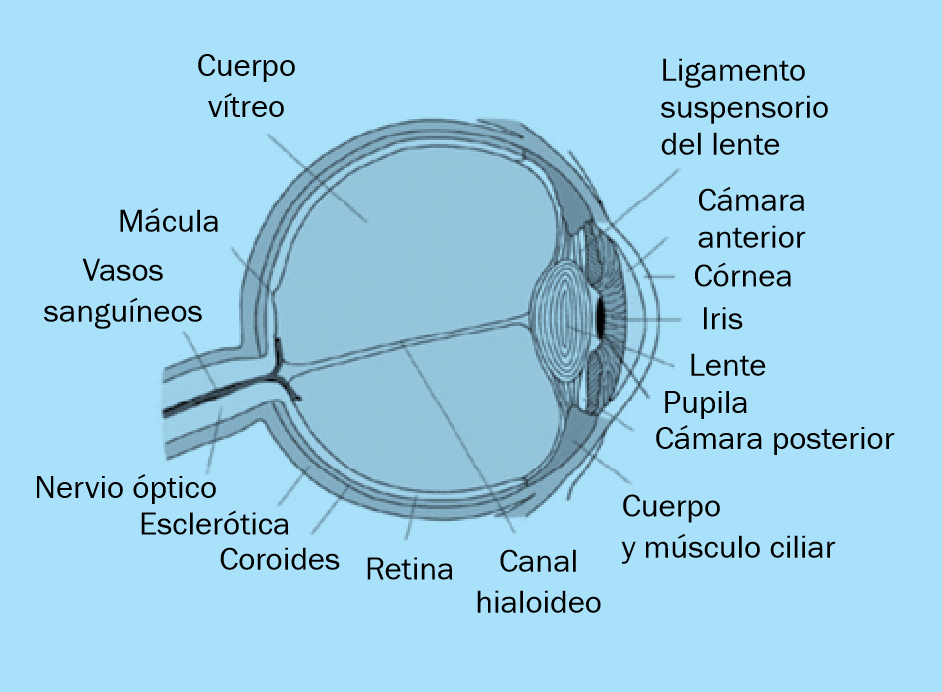
\includegraphics[width=0.45\textwidth]{imaxes/ojo1.png}
    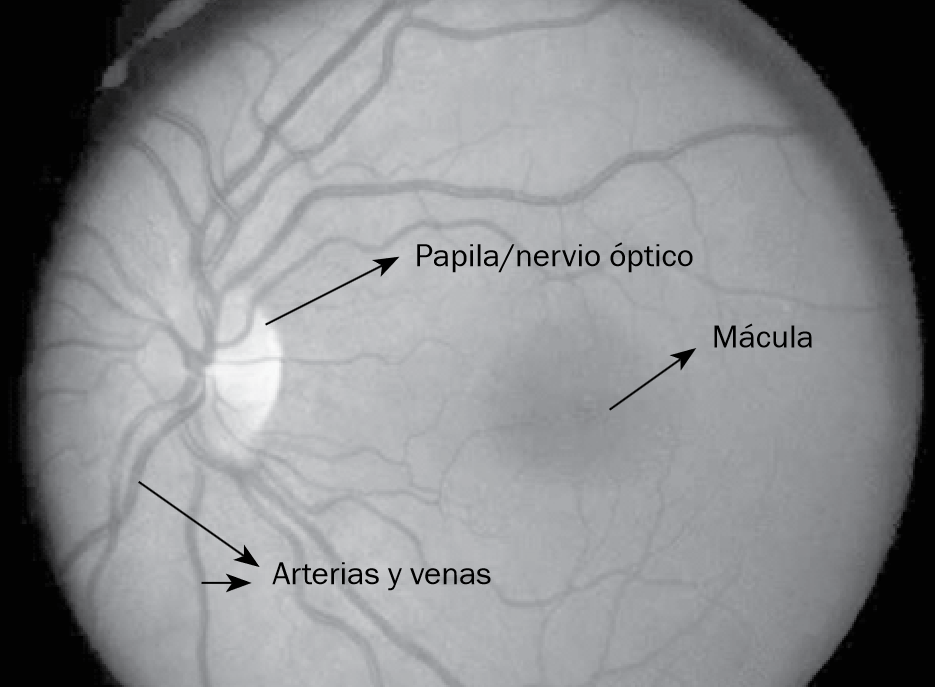
\includegraphics[width=0.45\textwidth]{imaxes/ojo2.png}
    \caption{Imaxes do ollo humano, extraídas de \cite{visionyojo}. Á esquerda, vista lateral do ollo anotada. Á dereita, retinografía do ollo anotada.}
    \label{fig:imaxes_ojo}
\end{figure}

\subsection{Imaxe oftalmolóxica}
\label{subsec:Imaxe oftalmolóxica}
Existen diversas modalidades de imaxe médica que permiten observar o ollo, cada unha con diferentes propiedades e aplicacións. 
Entre elas inclúense a fotografía de fondo de ollo, a tomografía de coherencia óptica (OCT) e a angiografía con fluoresceína \cite{ilginis2014ophthalmic}.

Este traballo céntrase na fotografía de fondo de ollo entre outras razóns polo seu uso común na práctica clínica.
Isto é débese en gran parte á súa accesibilidade, requerindo equipo máipólas barato e menor adestramento comparada cas outras modalidades. 
Ademais, é unha técnica non invasiva e rápida de realizar, o que a fai preferible na maioría dos casos \cite{retinimaging}.

Para realizala faise uso dunha cámara especial denominada retinógrafo, e xeralmente require da previa dilatación da pupila do paciente.
Desta forma permítese maior entrada de luz nos ollos, o que provoca unha mellor visualización da retina e mellora a calidade da imaxe.
Un especialista pode analizar a retinografía para detectar signos de enfermidades como a retinopatía diabética, a hipertensión ou a dexeneración macular \cite{retreggood}.

\section{Rexistro de imaxes}
\label{sec:Rexistro de imaxes}
O rexistro de imaxes é un proceso que consiste en, sobre dúas ou máis imaxes, determinar a correspondencia espacial entre elas
 e alinealas nun sistema de coordenadas común, co obxetivo de que as características de interese se atopen na mesma posición.

% Por exemplo, no caso do stitching de fotografías panorámicas, o rexistro de imaxes permite identificar correspondencias entre puntos característicos en múltiples tomas solapadas
%  e axustar a súa posición relativa nun marco común. Esta etapa é necesaria para a posterior fusión das imaxes, de modo que as distintas vistas se aliñen con precisión, producindo un resultado final continuo e sen irregularidades visuais.

O rexistro de imaxes ten utilidade en moitos campos diferentes como a imaxe satelital, xeografía, robótica... mais o 
campo da imaxe médica é dos máis interesantes pola súa aplicación práctica e é o que se aborda neste traballo \cite{goshtasby2017theory}.
Estas imaxes poden variar a nivel temporal, espacial, de dimensión ou de modalidade.

No ámbito da saúde un rexistro adecuado pode empregarse para comparar imaxes dun mesmo paciente tomadas en distintos momentos, en distintas modalidades ou para comparar entre diferentes pacientes.
Isto permite a revisión do avance dunha enfermidade ao longo do tempo, a fusión de imaxes de distintas modalidades ou a detección de patróns comúns entre distintos individuos.
A fusión de imaxes permite interpretar moito mellor a información dispoñible nelas, e é de gran axuda para guiar aos médicos na toma de decisións.
Tamén é útil para correxir os movementos involuntarios do paciente durante a adquisición de imaxes, como no caso da respiración en imaxes de pulmóns, ou para a intervención guiada por imaxe (\gls{IGRT}) que non 
podería funcionar sen a utilización axeitada de técnicas de rexistro de imaxes \cite{wang2022neuralrenderingstereo3d}. 

Ata recentemente, gran parte do traballo de rexistro facíase de forma manual por expertos con software como BigWarp \cite{bigwarp}, 
e dependía das habilidades do profesional para detectar as características de interese e realizar o aliñamento.
Isto facía que o proceso fose lento e propenso a erros, ademais de pouco práctico para grandes volumes de imaxes.

Na figura \ref{fig:retin_reg} móstrase un exemplo de rexistro de imaxes de retina, onde se pode observar como as imaxes son aliñadas para que as estruturas anatómicas coincidan.

\begin{figure}[tbp]
    \centering
    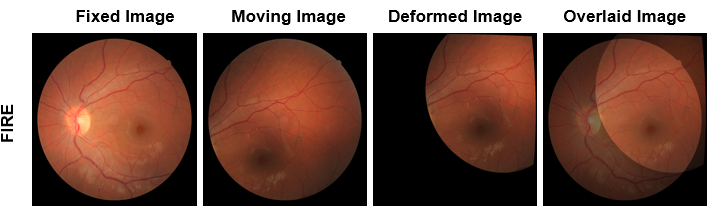
\includegraphics[width=0.8\textwidth]{imaxes/retin-reg.png}
    \caption{Exemplo de rexistro de imaxes de retina \cite{sivaraman2024retinaregnetzeroshotapproachretinal}}
    \label{fig:retin_reg}
\end{figure}

\subsection{Categorías de rexistro}
\label{subsec:Categorías de rexistro}

% O rexistro de imaxes pode ser clasificado en distintas categorías segundo as súas características. Na figura \ref{fig:categorias_de_rexistro} un resumo móstranse das categorías mais comúns.
O rexistro de imaxes pode ser clasificado en distintas categorías segundo as súas características.
% \begin{figure}[hp!]
%     \centering
%     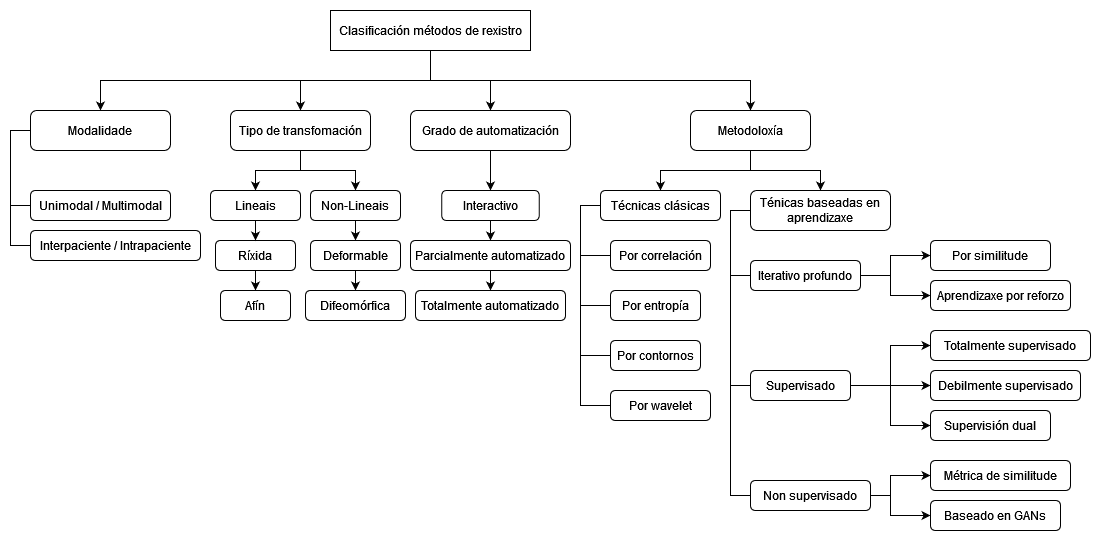
\includegraphics[width=1\textwidth]{imaxes/catreg.drawio.png}
%     \caption{Categorías de rexistro}
%     \label{fig:categorias_de_rexistro}
% \end{figure}

\begin{itemize}
    \item \textbf{Segundo o número de imaxes:}
    \begin{itemize}
        \item \textit{Par a par:} O rexistro realízase entre dúas imaxes, unha fixa e unha móbil.
        \item \textit{Múltiple:} Rexístranse varias imaxes simultaneamente, buscando unha correspondencia global.
    \end{itemize}

    \item \textbf{Segundo a modalidade:}
    \begin{itemize}
        \item \textit{Intra-modalidade:} As imaxes pertencen á mesma modalidade (por exemplo, dúas retinografías).
        \item \textit{Inter-modalidade:} As imaxes proveñen de modalidades diferentes (por exemplo, retinografía e OCT).
    \end{itemize}

    \item \textbf{Segundo o tipo de transformación:}
    \begin{itemize}
        \item \textit{Ríxida:} Só permite traslación e rotación, mantendo as distancias e ángulos.
        \item \textit{Afín:} Ademais de traslación e rotación, permite escalado e cizallamento.
        \item \textit{Deformable (non ríxida):} Permite deformacións locais complexas e non lineais.
        \item \textit{Difeomórfica:} Transformación non ríxida que é continua, invertible e diferenciable en todo o seu dominio. Se non ten esta característica, non se pode garantir que a transformación sexa reversíbel, polo que son preferidas en moitos casos \cite{han2022diffeomorphicimageregistrationneural}.
    \end{itemize}

    \item \textbf{Segundo o grao de automatización:} \cite{deeplernreview3dreg}
    \begin{itemize}
        \item \textit{Manual:} O usuario selecciona puntos de control ou axusta parámetros.
        \item \textit{Automático:} O proceso realízase sen intervención humana, mediante algoritmos.
        \item \textit{Semiautomático:} Combina intervención manual e automática.
    \end{itemize}

    \item \textbf{Segundo a natureza da transformación:}
    \begin{itemize}
        \item \textit{Simétrico:} A transformación é consistente en ambas direccións entre as imaxes.
        \item \textit{Asimétrico:} A transformación calcúlase só nun sentido. Cando se traballa con imaxes de forma asimétrica, a imaxe de referencia denomínase imaxe fixa e a imaxe que se quere rexistrar imaxe móbil.
    \end{itemize}

\end{itemize}

% \begin{itemize}
%     \item \textbf{Metodoloxía}
%     \begin{itemize}
%         \item \textbf{Técnicas clásicas} \cite{zitova2003imageregistrationsurvey}
%         \begin{itemize}
%             \item \textit{Por correlación:} Optimizan funcións de correlación entre as intensidades das imaxes para atopar a mellor aliñación.
%             \item \textit{Por entropía:} Baseados na maximización da información mutua, resultan especialmente útiles en rexistro multimodal.
%             \item \textit{Por contornos:} Empregan características xeométricas, como bordes ou liñas estruturais, para establecer correspondencias espaciais.
%             \item \textit{Por wavelet:} Utilizan descomposicións en diferentes frecuencias e resolucións para capturar información relevante.
%         \end{itemize}
        
%         \item \textbf{Técnicas baseadas en aprendizaxe} \cite{deeplernreview3dreg, bharati2022deeplearningmedicalimage}
%         \begin{itemize}
%             \item \textit{Iterativo profundo:} Estratexias que aplican redes neurais de forma recursiva para refinar progresivamente a transformación estimada.
            
%             \item \textbf{Aprendizaxe supervisada}
%             \begin{itemize}
%                 \item \textit{Totalmente supervisado:} Require datos de adestramento con aliñacións precisas (ground truth), que permiten optimizar directamente a tarefa de rexistro.
%                 \item \textit{Debilmente supervisado:} Emprega información parcial ou indirecta, como anotacións espaciais limitadas ou métricas proxy.
%                 \item \textit{Supervisión dual:} Combina diferentes formas de supervisión, como etiquetas explícitas e funcións de perda auto-supervisadas, para aumentar a xeneralización.
%             \end{itemize}
            
%             \item \textbf{Aprendizaxe non supervisada}
%             \begin{itemize}
%                 \item \textit{Métrica de similitude:} Optimiza criterios de similitude (e.g., NCC, SSIM) sen necesidade de datos anotados, favorecendo adaptación a novos dominios.
%                 \item \textit{Baseado en GANs:} Emprega arquitecturas adversarias para aprender transformacións realistas entre imaxes sen supervisión directa.
%             \end{itemize}
            
%             \item \textit{Por similitude:} Modelos que aprenden funcións de custo diferenciables que maximizan a coincidencia entre as imaxes de entrada.
%             \item \textit{Aprendizaxe por reforzo:} Formula o rexistro como un problema de toma de decisións, onde un axente aprende políticas óptimas mediante retroalimentación ambiental.
%         \end{itemize}
%     \end{itemize}
% \end{itemize}

As transformacións lineais globais soen representanse en matrices de transformación, onde cada elemento da matriz representa un parámetro da transformación.

No caso de transformacións máis complexas, utilízanse campos de vectores de deformación (\gls{DFV}s), que permite representar deformacións locais na imaxe, facendoa moito máis flexible para representar transformacións non lineais e detalladas.
Os DFVs adoitan ser representados cunha matriz de igual tamaño á imaxe, onde cada elemento representa un vector que indica a dirección e a magnitude da deformación.

Este traballo ubícase no rexistro de imaxes par a par, intra-modaliade e con transformacións deformables. É un proceso totalmente automático que produce transfomacións asimétricas.

Na figura \ref{fig:dfv_visualization} móstranse dúas formas de visualizar un DFV: mediante frechas que indican a dirección e magnitude da deformación, e aplicando a deformación a unha cuadrícula para ver como se distorsiona.

\begin{figure}[tbp]
    \centering
    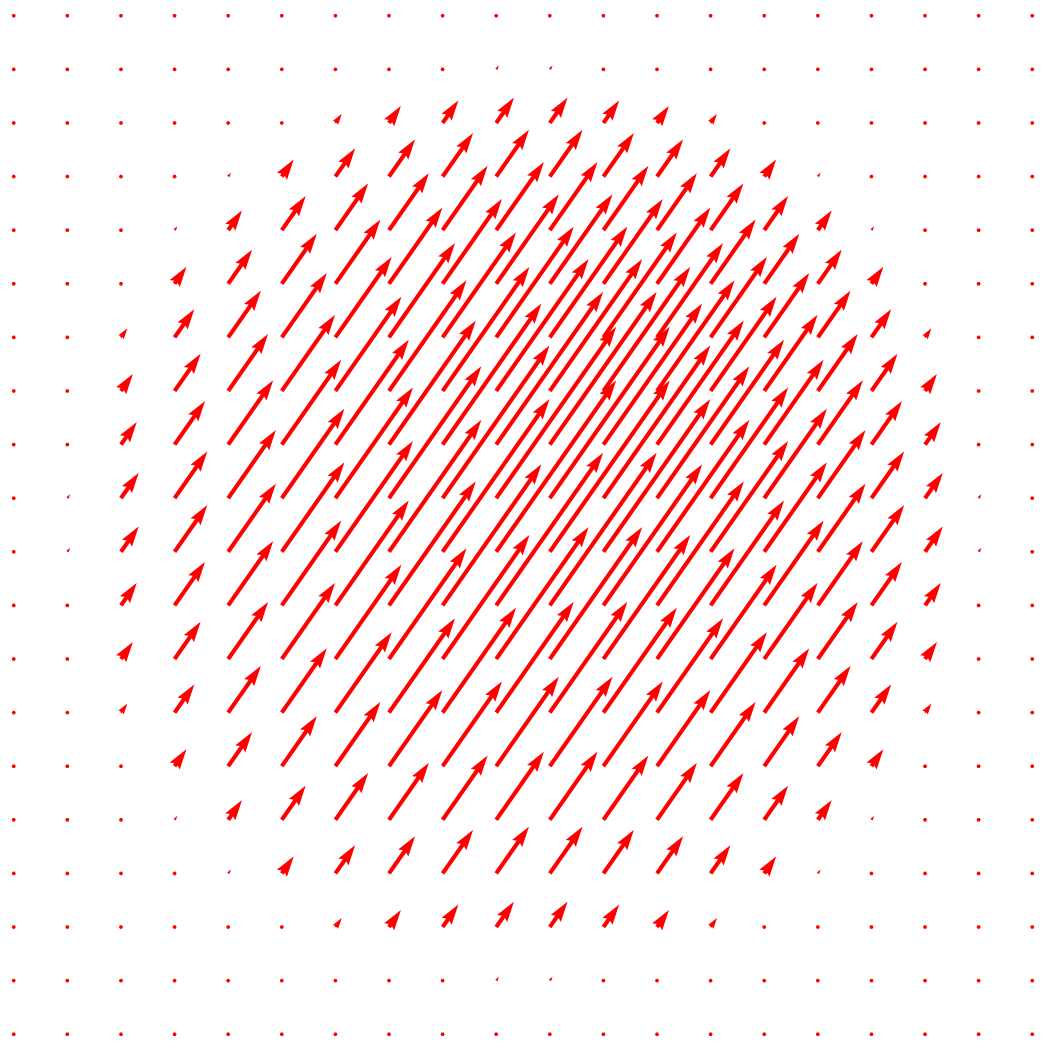
\includegraphics[width=0.45\textwidth]{imaxes/dfv_arrows.png}
    
\includegraphics[width=0.45\textwidth]{imaxes/dfv_grid.png}
    \caption{Visualización do campo de vectores de deformación (DFV). Á esquerda, representación mediante frechas. Á dereita, esta deformación aplicada a unha cuadrícula.}
    \label{fig:dfv_visualization}
\end{figure}

\subsection{Estado da arte}
\label{subsec:Estado da arte}

% Pese á gran cantidade de avances que está a ocorren no campo do aprendizaxe profunda, os métodos clásicos de rexistro de imaxes seguen a ser o estado do arte na maioría de casos,
% principalmente debido á importancia da precisión e a robustez en imaxe médica.

O rexistro de imaxes médicas constitúe unha área de investigación fundamental que experimentou importantes avances nas últimas décadas. Neste ámbito, a precisión e a robustez do rexistro cobran especial relevancia, xa que son empregados para o diagnóstico e seguimento de enfermidades, así como para a planificación de tratamentos cirúrxicos.
No eido da oftalmoloxía, os métodos que funcionan ben en varios dominios de imaxe médica (cerebro, pulmóns, etc) adoitan requirir de axustes para funcionar en retinas, polo que hai un estado da arte paralelo. 

A evolución dos métodos de rexistro en retinografías reflicte a transición dende enfoques puramente algorítmicos cara metodoloxías híbridas, onde publicacións recentes como HybridRetina \cite{liu2024progressiveretinalimageregistration}  mostran como para acadar os mellores resultados é beneficioso combinar ambos enfoques, aproveitando a precisión dos métodos clásicos e a adaptabilidade dos métodos de aprendizaxe automático.

\subsubsection{Métodos clásicos}
\label{subsubsec:Métodos clásicos}

Os métodos clásicos de rexistro de imaxes médicas poden clasificarse en dúas categorías principais:
Aqueles baseados en similitude de imaxe (\gls{IBR}) e aqueles baseados en características (\gls{FBR}).
Tamén existen métodos híbridos que combinan ambos enfoques \cite{integrateintfeat}.
O resultado final pode ser os parámetros da transformación ou a imaxe fusionada.

\paragraph{Métodos baseados en similitude de imaxe}
\label{par:Métodos baseados en similitude de imaxe}

O rexistro realízase comparando os valores de intensidade dos píxeles ou voxeles mediante unha métrica de similitude entre a imaxe fixa e a imaxe móbil.
Este enfoque tende a requerir de múltiples iteracións para converxer, nas cales calcúlase o grado de semellanza entre as imaxes e
actualízanse os parámetros da transformación utilizando un mecanismo de optimización ata que se cumpran os criterios de terminación.

Os métodos de rexistro tradicionais teñen tres compoñentes principais: a métrica de similitude, o optimizador e o modelo de transformación. 

A figura \ref{fig:rexistro_iterativo} mostra un diagrama do proceso de rexistro iterativo.

% ejemplos?

\paragraph{Métodos baseados en características}
\label{par:Métodos baseados en características}

O rexistro realízase identificando e emparellando características salientables entre as imaxes, como puntos, liñas ou bordes.
Tipicamente, estes métodos teñen 3 pasos principais:

\begin{itemize}
\item \textbf{Detección de puntos de interese:} Identificación de puntos ou rexións salientables nas imaxes, como bordes, esquinas ou texturas. Para isto poden utilizarse utilízanse algoritmos como SIFT \cite{sift}, SURF \cite{surf}, BRISK \cite{brisk} ou FREAK \cite{freakkeypoint}.
\item \textbf{Descrición de características:}  os puntos detectados son descritos e comparados entre imaxes usando descritores .
\item \textbf{Estimación da transformación:} unha vez atopadas as correspondencias, calcúlase a transformación que aliña as imaxes con algoritmos de emparellamento como FLANN \cite{flann} ou RANSAC \cite{ransac}.
\end{itemize}

Algúns dos métodos tradicionalmente máis utilizados neste campo son \gls{GDB-ICP} \cite{GDB-ICP} e Harris-PIIFD \cite{piifd}. Este último utiliza o algoritmo Harris \cite{Harris1988ACC} para a detección de puntos de interese, descríbenos con \gls{PIIFD}, e emparéllanse usando \gls{BBF} \cite{BBF}.
 Finalmente, refínanse as coincidencias e escóllese a transformación (ríxida, afín ou polinomial) segundo o número de pares de puntos válidos. Sobre esta base propuxéronse varias melloras para adaptalo ao rexistro multimodal de retinas como UR-SIFT \cite{ur-sift} ou \gls{GMM} \cite{GMM}.

Unha vantaxe deste enfoque é a capacidade para rexistrar imaxes con grandes variacións locais ou modalidades diferentes, xa que non depende tanto da semellanza global entre as imaxes.

Outros métodos clásicos relevantes no campo da imaxe de ollo inclúen REMPE \cite{rempe}, que estima simultaneamente a pose das cámaras e a forma do ollo. Fai uso de un modelo elipsoidal para o ollo e estima a posición das cámaras con RANSAC, para logo refinala cunha variante de PSO \cite{pso}. 
% Versións anteriores deste método utilizaron modelos esféricos e \gls{SURF} no canto de SIFT \cite{H-M16}.

\begin{figure}[tbp]
\centering
\begin{tikzpicture}[node distance=2cm, scale=0.8, every node/.style={transform shape}]
% Nodes
\node (imageFixa) [process] {Imaxe Fixa};
\node (imageMobil) [process, right of=imageFixa, xshift=3cm] {Imaxe Móbil};
\node (featureExtraction) [process, below of=imageFixa, yshift=-1cm] {Cálculo de medida de similitude};
\node (parameterUpdate) [process, below of=featureExtraction, yshift=-1cm] {Actualización de Parámetros};
\node (applyTransformation) [process, below of=parameterUpdate, yshift=-1cm] {Aplicar a Transformación};
\node (criteriaCheck) [decision, below of=applyTransformation, yshift=-1cm] {Criterios Cumpridos?};
\node (result) [process, below of=criteriaCheck, yshift=-1cm] {Resultado};
% Arrows
\draw [arrow] (imageFixa) -- (featureExtraction);
\draw [arrow] (imageMobil) -- (featureExtraction);
\draw [arrow] (featureExtraction) -- (parameterUpdate);
\draw [arrow] (parameterUpdate) -- (applyTransformation);
\draw [arrow] (applyTransformation) -- (criteriaCheck);
\draw [arrow] (criteriaCheck) -- node[anchor=west] {Sí} (result);
\draw [arrow] (criteriaCheck.east) -- ++(1,0) node[anchor=south, xshift=0.5cm] {No} |- (featureExtraction.east);
\end{tikzpicture}
\caption{Proceso de rexistro de imaxes iterativo}
\label{fig:rexistro_iterativo}
\end{figure}

Tamén existen múltiples programas que fan uso de estos métodos en ferramentas para facilitar o rexistro de imaxes, como SimpleITK \cite{simpleitk}, Elastix \cite{elastix} ou ANTs \cite{ants}.

\subsubsection{Métodos de aprendizaxe profunda}
\label{subsubsec:Métodos de aprendizaxe profunda}

Coa chegada dos métodos de aprendizaxe profunda á imaxe médica, comezaron a empregarse redes neuronais para realizar o aliñamento de imaxes.
Existe un gran interés polos métodos baseados en aprendizaxe profundo, como se reflexa no crecente número de publicacións no campo. Na figura \ref{fig:method_comp} móstrase a evolución do número de publicacións sobre rexistro de imaxes, diferenciando entre os métodos baseados en aprendizaxe profunda e os métodos tradicionais.

% Estos métodos tenden a ser mais rápidos que os métodos convencionais, a custo de algo de precisión.
Os métodos de aprendizaxe profunda poden ser clasificados en dous tipos según se requiran de \glossary{DFV}s anotados ou non na etapa de adestramento:
supervisados (requíren anotacións) e non supervisados (non requíren anotacións) \cite{nie2024medicalimageregistrationapplication}.

Segundo o grado de supervisión utilizado na etapa de adestramento, os métodos supervisados poden dividirse en supervisados ou débilmente supervisados.
O rexistro totalmente supervisado fai uso de DVFs de referencia para supervisar o proceso de aprendizaxe, e o termo de perda adoita basearse na discrepancia entre os DVFs de referencia e os DVFs predicidos.

O rexistro débilmente supervisado pode utilizar outras etiquetas de referencia implícitas, non baseadas en datos explícitos como os DFVs, senón que utilizan información indirecta para guiar o proceso de rexistro, como a semellanza entre as imaxes ou restricións baseadas na forma ou límites anatómicos das estruturas.
Máis de dous tipos de datos de referencia son frecuentemente utilizados para adestrar modelos de rexistro débilmente supervisados \cite{bharati2022deeplearningmedicalimage}.

Os métodos non supervisados teñen a vantaxe de non requirir de datos anotados, o cal é unha gran vantaxe xa que un dos maiores retos para as redes de imaxes médicas é a recolección de datos de calidade para o adestramento \cite{medicalimageanalysis}.
A creación de conxuntos de DFVs anotados é un proceso laborioso e costoso, que normalmente sólo póde ser executado por especialistas, polo que os métodos de rexistro non supervisados son de gran interese.
De forma similar aos métodos iterativos, é común empregar unha métrica de similitude entre as imaxes xunto con un termo de regularización para guiar o proceso de optimización evitando caer en transformación non realistas.
% Xa que a imaxe fixa e a imaxe móbil xa conteñen toda a información necesaria para un rexistro correcto, os métodos non supervisados parecen mais adecuados para a tarefa de rexistro.

Os enfoques de aprendizaxe profundo son útiles tanto na súa capacidade de aprender a tarefa de rexistro de maneira end-to-end, como para substituír módulos concretos do proceso tradicional.
Nese sentido, os métodos de aprendizaxe profunda poden ser categorizados según a tarefa do proceso de rexistro que substitúen.

\begin{figure}[tbp]
\centering
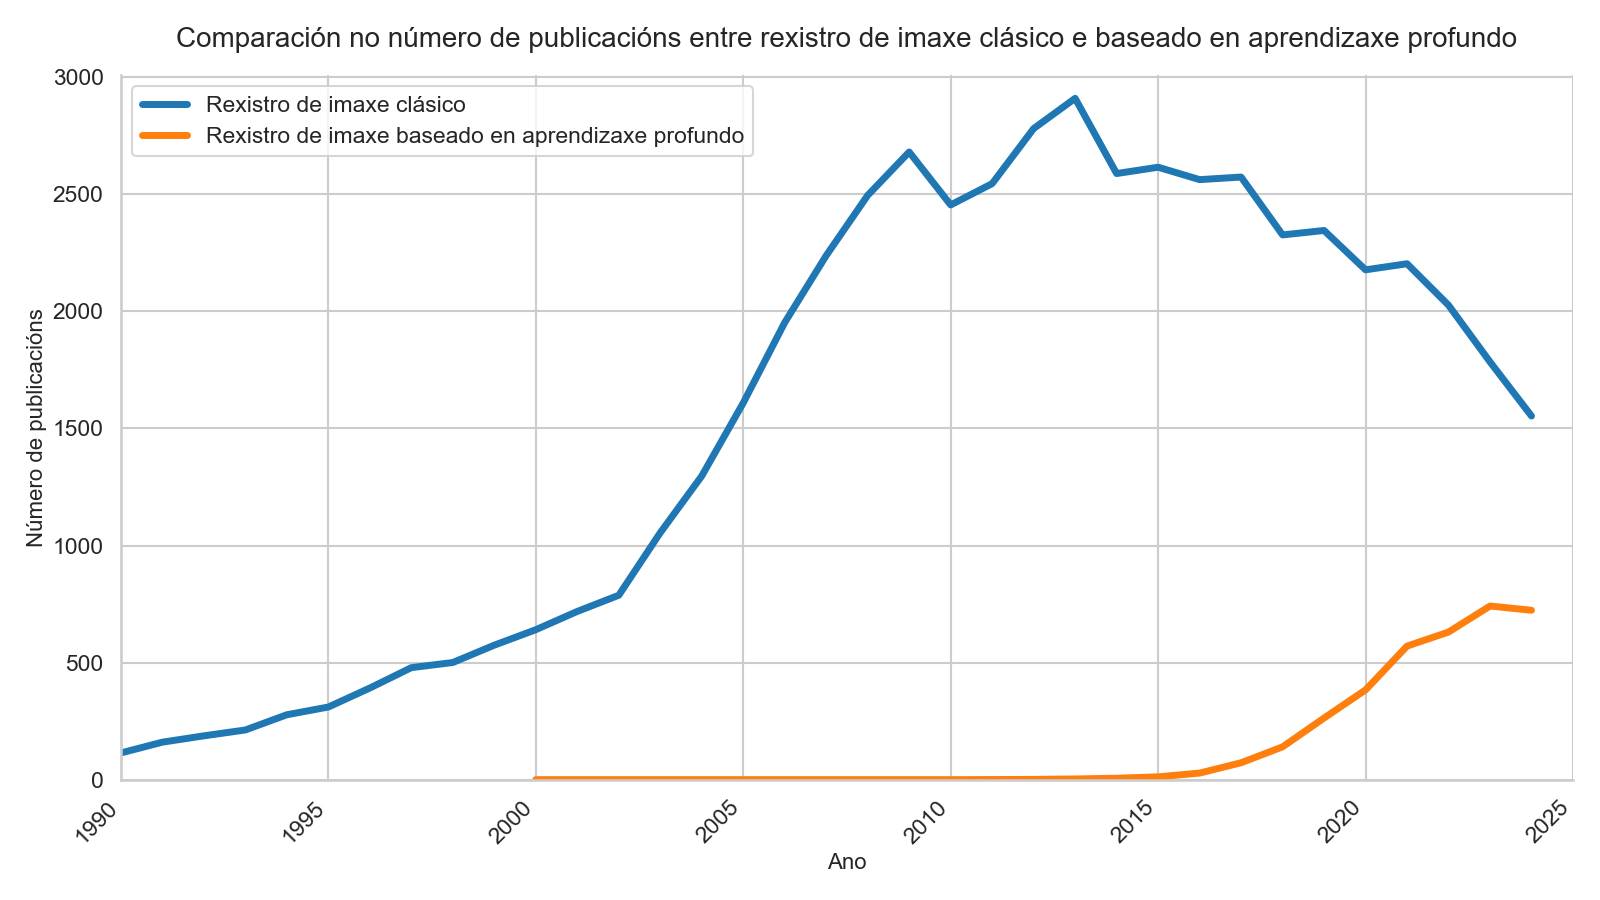
\includegraphics[width=0.8\textwidth]{imaxes/methods_comp.png}
\caption{Comparación de pubicacións ó longo do tempo que relacionadas co rexistro de imaxes. Datos extraídos de Scopus \cite{scopus}, realizando as consultas: "TITLE-ABS-KEY(image AND registration) AND NOT(deep AND learning)" e "TITLE-ABS-KEY(image AND registration) AND (deep AND learning)"}
\label{fig:method_comp}
\end{figure}

Os métodos de aprendizaxe profunda poden substituír calquera destes pasos que forman os métodos de rexistro clásicos de forma independente ou en combinación.

\paragraph{En rexistro baseado en intensidade (IBR)}
\label{par:IBR_substitution}

\begin{itemize}
\item \textbf{Métrica de similitude:} Os métodos de aprendizaxe profunda poden aprender métricas de similitude máis robustas que as tradicionais. Estas métricas aprendidas poden ser máis efectivas en imaxes multimodais ou con artefactos.
Por exemplo, Czolbe et al. \cite{semanticsimilarity} propoñen dúas métricas de similitude semánticas que aprende a semellanza entre imaxes comparando as características de alto nivel extraídas. Presentan unha aproximación non supervisada que fai uso de autoencoders e outra semisupervisada que incorpora datos de segmentación.
\item \textbf{Optimizador:} Os métodos de aprendizaxe profunda poden substituír o proceso de optimización iterativa tradicional por redes que aprenden a predicir directamente os parámetros de transformación óptimos. Unha aproximación común é empregar estes conxuntos de datos para optimizar unha CNN que, dadas dúas imaxes novas e non vistas, predí o DFV correspondente \cite{defregcnn}. Durante o proceso de adestramento, a rede pode ter acceso aos DFVs coa deformación correcta, ou pódense obter indirectamente a través da optimización dunha métrica de similitude de imaxes.
\item \textbf{Modelo de transformación:} Estes métodos aprenden representacións implícitas da transformación a través de redes neuronais, permitindo modelar deformacións máis complexas que os modelos paramétricos tradicionais. Os métodos como IDIR \cite{wolterink2021implicit} encaixan nesta categoría, utilizando campos neuronais implícitos para representar as transformacións de rexistro.
\end{itemize}

% Existen diferentes extensións a esta aproximación, como o uso de múltiples etapas ou o uso de redes adversarias durante o adestramento.

% Tamén se propuxeron métodos híbridos que combinan a optimización iterativa ca aprendizaxe profunda,
% entrenando unha CNN nova por cada parella de imaxes. Desta forma conséguese evitar a necesidade de grandes conxuntos de datos para o adestramento.

\paragraph{En rexistro baseado en características (FBR)}
\label{par:FBR_substitution}

\begin{itemize}
\item \textbf{Detectores de características:} As redes neuronais poden aprender a detectar puntos de interese máis robustos e repetibles que os detectores clásicos como \glossary{SIFT}. SuperPoint \cite{superpoint} introduce un detector de características baseado en redes neuronais que aprende a detectar puntos de interese e a describilos simultaneamente.
\item \textbf{Descriptores de características:} Os descriptores aprendidos mediante redes neuronais poden capturar información máis discriminativa, mellorando a precisión do emparellamento posterior. Estes métodos aprenden representacións que son invariantes a transformacións específicas do dominio.
\item \textbf{Emparellamento:} As redes neuronais poden aprender a realizar o emparellamento de características de forma robusta, especialmente en presenza de cambios de iluminación ou perspectiva. SuperGlue \cite{superglue} é un exemplo de modelo que aprende a emparellar puntos de interese detectados utilizando unha arquitectura baseada en atención para capturar as relacións entre os puntos.
\end{itemize}

\paragraph{Métodos de regresión directa}
\label{par:direct_regression}

A aprendizaxe profunda tenden a requerir dunha gran cantidade de datos para ser adestrados, o que pode ser unha desventaxa xa que en moitos casos non se dispoñen de bases de datos anotadas do tamaño necesario.

Os métodos de regresión directa aprenden a mapear directamente desde un par de imaxes ata os parámetros da transformación, sen necesidade de optimización iterativa nin extracción explícita de características.

Tamén son denominados métodos de inferencia amortizada debido á capacidade de realizar múltiples inferencias (rexistros) tras un único proceso de adestramento, en contraposición aos métodos tradicionais que requiren optimización individual para cada par de imaxes.
Estes enfoques son útiles pola súa eficiencia computacional na fase de inferencia. Voxelmorph \cite{Balakrishnan_2019voxelmorph} é un dos frameworks máis utilizados no rexistro de imaxes deformable, facendo uso de modelos baseado en \gls{CNN}s e que tamén permite incorporar información auxiliar (como segmentacións) se está dispoñible, mellorando así a precisión do rexistro.

Métodos como UDIR-Net \cite{undefreg} ou DIO \cite{Jena_2025} tamén implementan estas ideas.

% \paragraph{GANs}
% \label{par:GANs}

% As \gls{GAN} (Generative Adversarial Network) son un tipo de rede neuronal que consta de dous modelos que compiten entre si: un xerador e un discriminador. O xerador intenta crear datos falsos que sexan indistinguibles dos datos reais, mentres que o discriminador intenta distinguir entre os datos reais e os datos xerados. Este proceso de competición mellora iterativamente a calidade dos datos xerados e o criterio do discriminador.

% No contexto do rexistro de imaxes, as GANs poden ser utilizadas para aprender a transformación entre imaxes de forma non supervisada. O xerador pode ser adestrado para producir transformacións que aliñen a imaxe móbil coa imaxe fixa, mentres que o discriminador avalía a calidade do rexistro.
% Un exemplo de aplicación de GANs no rexistro de imaxes médicas é o traballo de Mahapatra et al. \cite{mahapatra2019ganbasedmedicalimage}, onde se propón un modelo de rexistro de imaxes baseado en GANs que demostrou ser efectivo tanto en retinas como con resonancias magnéticas cardiovasculares.

\subsubsection{Estado da arte no rexistro de retinografías}
\label{subsubsec:Estado_da_arte_no_rexistro_de_retinografías}

O rexistro de retinografías presenta un conxunto de desafíos únicos que o distinguen doutros dominios da imaxe médica.
Un dos principais obstáculos son as deformacións non ríxidas. Estas deformacións poden orixínarse pola proxección da superficie 3D curva da retina nunha imaxe 2D ou variacións na forma do ollo de cada paciente. Ademais, é frecuente atopar pares de imaxes con áreas de solapamento mínimas o que dificulta a identificación de correspondencias para o aliñamento. A isto súmanse as variacións de iluminación, contraste e cor entre imaxes capturadas en diferentes situacións, así como os cambios anatómicos inducidos por patoloxías, que alteran as estruturas utilizadas para o rexistro. 
Finalmente, a escaseza de conxuntos de datos públicos, especialmente para condicións ou poboacións específicas, supón unha barreira importante para o desenvolvemento de modelos de aprendizaxe supervisada.    

A dificultade para obter campos de deformación de referencia para o adestramento impulsou o desenvolvemento de marcos non supervisados. Estes modelos adéstranse optimizando unha función de perda baseada na similitude de imaxe entre a imaxe móbil deformada e a imaxe fixa, xunto cun termo de regularización sobre a suavidade da deformación. 

% A figura \ref{tab:retina_reg_comp} mostra unha análise comparativa revela un claro compromiso entre precisión e velocidade. Métodos clásicos como REMPE poden acadar unha alta precisión, pero son computacionalmente moi custosos (p. ex., 198 segundos por par de imaxes). En contraste, os métodos de aprendizaxe profunda son ordes de magnitude máis rápidos (p. ex., 0.65 segundos por par), aínda que poden sacrificar parte da precisión nos casos máis complexos. A seguinte táboa resume esta comparativa.  

Dentro dos métodos clásicos, os baseados en características (FBR) seguen a ser referentes en canto a precisión. Entre eles destacan VOTUS \cite{Votus}, que é especialmente robusto en imaxes de pouco solapamento e representa as árbores vasculares como grafos para atopar a correspondencia entre eles. REMPE \cite{rempe} é outro método xa mencionado anteriormente nesta categoría.

No campo da aprendizaxe profunda, RetinaRegNet \cite{sivaraman2024retinaregnetzeroshotapproachretinal} é un modelo recente que de tipo "zero-shot" que utiliza características extraídas de modelos de difusión para establecer correspondencias, acadando resultados de vangarda

%  \cite{ConKeD}  \cite{ConKeD2}
ConKeD (Contrastive Keypoint Descriptors) e a súa evolución, ConKeD++ , céntranse en perfeccionar a creación de descritores de puntos de interese, un dos compoñentes máis críticos dos métodos baseados en características (FBR).
A principal vantaxe é que obtén resultados comparables aos dos métodos clásicos de vangarda (como REMPE e VOTUS) pero con tempos de execución moito máis rápidos

A maioría destes algoritmos son avaliados e comparados utilizando o conxunto de datos de referencia FIRE \cite{FIRE}, permitindo unha cuantificación obxectiva do rendemento.

\section{Representación Neuronais Implícitas}
\label{sec:Representación Neuronais Implícitas} 

A representación de coñecemento é un dos problemas máis importantes na área da computación, e as 
redes profundas son unha das ferramentas máis útiles, especialmente no campo da visión por computador.
Tradicionalmente empréganse representacións discretas, onde o espazo de entrada é dividido en celdas e cada celda é asignada un valor (por exemplo nubes de puntos, matrices de píxeles ou vóxeles...).
Unha das principais desventaxas destas representacións é que a súa complexidade increméntase rápidamente co número de dimensións representadas, ademais do custo de memoria asociado.

 As representacións neuronais implícitas son un paradigma innovador que permite modelar sinais continuas mediante funcións parametrizadas por redes neuronales.
 Codifican a información como unha función continua, que mapea valores de entrada aos valores correspondientes de saída, en lugar de almacenar directamente valores de características o señales.

Representar o sinal como una función continua permite solucionar os problemas asociados á discretización e obtéñense outra serie de vantaxes.

As INR son moito mais eficientes debido á compresión da información que realizan de forma implícita. Ao mesmo tempo, permite un nivel de detalle non limitado pola resolución da imaxe, senón pola capacidade da rede. 
 Ademais, as representacións continuas son diferenciables, o que permite o cálculo de gradientes e derivadas de forma analítica en lugar de ter que aproximalos por diferencias finitas.
 Isto tamén implica que as representacións implícitas son independentes da resolución, o que permite a reconstrucción en calquera escala espacial.
 
Tipicamente emprégase un MLP como architectura para representar a función implícita. Non obstante, o uso da función de activación ReLU tende a non obter os mellores resultados, debido a que son incapaces de representar deformacións locais sen afectar o sea comportamento global \cite{rahaman2019spectralbiasneuralnetworks},
polo que moita investigación diríxese a atopar alternativas que melloren a representación do sinal. \cite{essakine2024standimplicitneuralrepresentations}

Unha destas alternativas é SIREN \cite{sitzmann2020implicitneuralrepresentationsperiodic}, sobre a que profundizaremos máis adiante.
Outras propostas inclúen \cite{ramasinghe2022periodicityunifyingframeworkactivations} propón as funcións de activación gaussianas como alternativa a SIREN, e argumenta que poden obter mellores representacións e máis robustas.
\cite{saragadam2023wirewaveletimplicitneural} achega unha nova función de activación baseada en wavelets, que parece ser especialmente útil para a representación de imaxes.

As representacións implícitas poden ser clasificadas en dúas categorías: xeneralizables e sobreaxustadas \cite{yu2024neuraltrajectorymodelimplicit}. 
As representacións sobreaxustadas céntranse en reproducir con precisión unha única sinal, mentres que as representacións xeneralizables poden modelar varias nunha mesma rede.

\subsection{Aplicacións}
\label{subsec:Aplicacións}

As INR son utilizadas en todo tipo de campos, dende xeración de imaxes \cite{reddy2022multiimplicitneuralrepresentationfonts}, pasando por
reconstrucción de obxetos \cite{mildenhall2020nerfrepresentingscenesneural} \cite{mescheder2019occupancynetworkslearning3d} ou modelado de sinais complexas \cite{wu2021iremhighresolutionmagneticresonance}.

As representacións implícitas están a recibir cada vez máis atención da comunidade médica, e son 
especialmente útiles para as tarefas de imaxe inversa, que requiren a reconstrucción de representacións correctas a partir de datos incompletos ou ruidosos \cite{molaei2023implicitneuralrepresentationmedical}. 
Métodos como NeRP, propuxeron o uso de representacións implícitas para a reconstrucción de imaxes de resonancia magnética a partir de datos incompletos, 
e obtiveron resultados comparables a métodos tradicionais \cite{shen2023nerpimplicitneuralrepresentation}.

NeRF fai uso de representacións implícitas para a sintetizar novos puntos de vista en escenas 3D  \cite{mildenhall2020nerfrepresentingscenesneural}, 
 optimizando unha función volumétrica continua que modela a densidade de volume e a radiancia emitida en cada punto do espazo.
 Utilizan un MLP, cuxa entrada é unha única coordenada continua 5D (localización espacial (x, y, z) e dirección de visión (θ, φ)) 
 e cuxa saída é a densidade de volume e a radiancia emitida dependente da vista nesa localización espacial. 
A única entrada necesaria para optimizar a súa representación é un conxunto de imaxes con poses de cámara coñecidas. 
Este traballo demostra que as representacións implícitas están capacitadas para modelar escenas 3D complexas con alta fidelidade visual.
 
As representacións implícitas tamém teñen bastante potencial no campo de planificación de traxectorias, 
onde se fai uso de INRs para modelar entornos e planificar traxectorias para un ou varios axentes \cite{yu2024neuraltrajectorymodelimplicit}.
A principal vantaxe de facelo desta forma frente á forma tradicional (algoritmos computacionalmente intensos, especialmente para multi-axentes) é a velocidade á que encontran solucións (por debaixo do milisegundo en GPUs).
A maior desventaxe é que non garanten a converxencia a unha solución óptima e sen colisións, mais os autores demostran que a calidade das traxectorias xeradas é adecuada para a maioría das aplicacións \cite{trajectinr}.

No ámbito médico, utilizanse este tipo de representacións para garantir a seguridade do paciente durante a cirurxía teleoperada e optimizar a traxectoria do robot para evitar colisións co paciente, por exemplo nas boca e gorxa \cite{teleoperatdrob}.
Con este método, evítase a reconstrución de mallas a partir de imaxes, que é un proceso costoso e imperfecto, e modélase mediante unha INR a partir dos datos médicos dispoñibles.
Os comandos de movemento da man do operador son tomados como entrada polo modelo, que logo de un proceso de optimización, xera unha secuencia de movementos libre de colisións que será enviada á man robótica.
Tamén son utilizadas para crear reconstruccións 3D de pulmóns que mitigan as distorsións causadas polo movemento respiratorio \cite{velikova2024implicitneuralrepresentationsbreathingcompensated}.

Outro uso interesante das representacións neuronais implícitas é a compresión de imaxes. Algoritmos como COIN \cite{coin} representan os datos de entrada mediante redes neuronais implícitas (funcións que mapean coordenadas a valores RGB), logrando unha compresión eficiente e unha redución significativa do tempo de codificación en moitas modalidades.

\subsection{Rexistro baseado en Representacións Neuronais Implícitas}
\label{subsec:Rexistro_baseado_en_INRs}

O rexistro de imaxes baseado en Representacións Neuronais Implícitas (INR) parametriza a transformación de deformación como unha función continua, xeralmente cun Perceptrón Multicapa (MLP), que mapea coordenadas espaciais a vectores de desprazamento. A diferenza das CNN, a rede non procesa as intensidades da imaxe directamente, senón que se optimiza usando estas para calcular a perda. Unha das vantaxes neste contexto é a capacidade de calcular gradientes analíticos exactos da transformación, permitindo unha regularización máis precisa que con aproximacións dos métodos baseados en grellas.  

As funcións de activación periódicas (SIREN \cite{sitzmann2020implicitneuralrepresentationsperiodic}) permitiron sobrepasar o problema dos sesgos cara transformacións de baixa frecuencia do MLP, e foron utilizadas por IDIR acadando resultados de vangarda \cite{wolterink2021implicit}.  

Os principais inconvenientes son a lentitude na inferencia (require optimización para cada par de imaxes) e a tendencia a xerar pregamentos espaciais (deformacións non realistas). A investigación actual céntrase en modelos híbridos para mitigar estes problemas.
Algúns dos enfoques máis relevantes inclúen:
SINR (Spline-enhanced INR) combina INR con B-splines, onde a rede predí os desprazamentos dunha grella de control dispersa. Isto impón suavidade de forma intrínseca e facilita o rexistro multimodal \cite{SINR}.   
INR ciclo-consistentes, que adestran simultaneamente a transformación directa e a inversa, usando cada rede como regularizador da outra para mellorar a robustez.  
Meta-aprendizaxe: Aprende unha inicialización de pesos óptima a partir dun gran conxunto de datos para acelerar drasticamente a converxencia na inferencia \cite{learnedinit}.  
INR condicionadas por xeometría: Incorporan coñecemento anatómico previo para simplificar a complexidade da deformación a aprender \cite{harten2023deformable}.  
Sun et al. \cite{sun2024medicalimageregistrationneural} propóñen un rexistro de imaxes que usa campos neuronais para modelar a transformación, utilizando tamén codificación posicional (que transforma a coordenadas espaciais en vectores de alta dimensión) o que permite que a rede aprenda con maior facilidade as transformacións de alta frecuencia.

O uso de Representacións Neuronais Implícitas (INR) para o rexistro de imaxes ofrece unha precisión notable ao modelar a deformación como unha función continua e analiticamente diferenciable. Este enfoque, exemplificado polo éxito inicial de IDIR, permite unha regularización máis exacta que os métodos baseados en grellas. Non obstante, a súa aplicación práctica vese obstaculizada pola lentitude da optimización por cada par de imaxes e o risco de producir deformacións non realistas con pregamentos espaciais. O estado da arte actual tende a abordar estes retos mediante a hibridación.

\section{Traballo proposto}
\label{sec:Traballo proposto}

O traballo proposto ubícase dentro do dos métodos de aprendizaxe profunda, e máis concretamente no rexistro de imaxes baseado en intensidade (IBR) utilizando representacións neuronais implícitas (INRs).

Como mostramos neste capítulo, a pesar do potencial das representacións neuronales implícitas en diversos dominios médicos, a súa aplicación específica ao rexistro de retinografías permanece inexplorada.

Este falta de investigación é especialmente relevante dadas as potenciais vantaxes que ofrecen as INRs, como a capacidade de modelar deformacións complexas e a súa independencia da resolución.

Baseándose no framework introducido por \cite{wolterink2021implicit}, propónse modificalo para adaptalo á tarefa de rexistro de retinografías. O obxetivo é conseguir rexistros consistentemente precisos, especialmente no dataset de FIRE que contén imaxes reais de retina.

Esta adaptación representa unha contribución novel ao estado da arte no rexistro de retinografías, explorando por primeira vez o potencial das representaciones neuronales implícitas neste dominio específico.

 \chapter{Metodoloxía e planificación}
\label{chap:Metodoloxía e planificación}
\lettrine{N}{esta} sección explícase a metodoloxía de traballo empregada para o desenvolvemento do proxecto, así como a planificación do mesmo.
 Ademais, descríbense os recursos utilizados e faise unha estimación dos custos asociados ao proxecto.

\section{Metodoloxía do desenrolo}
\label{sec:Metodoloxía do desenrolo}

Ao ser un proxecto de investigación, a metodoloxía de traballo máis adecuada é unha metodoloxía iterativa e incremental, que permite poder adaptarse aos cambios que van xurdindo durante o desenrolo do proxecto.
Esta metodoloxía permite obter un artefacto funcional ao final de cada iteración, o que permite obter retroalimentación constante sobre o desenrolo do proxecto.
Cada iteración comeza cunha análise do que se quere conseguir, seguida das fases de deseño e codificación, e remata cunha fase de testeo do produto desenvolvido.

\section{Planificación do proxecto}
\label{sec:Planificación do proxecto}
O proxecto inicialmente divídese nas seguintes fases principais:

\begin{itemize}
    \item \textbf{Revisión do estado da arte:}
    \begin{itemize}
        \item Estudo do dominio biolóxico: características das imaxes oftalmolóxicas, a súa importancia e aplicacións.
        \item Análise de traballos relacionados con IDIR, representacións implícitas e segmentación de imaxes oftalmolóxicas mediante redes neuronais.
    \end{itemize}
    Esta fase estimouse en aproximadamente 3 semanas de traballo, dada a necesidade de familiarizarse co contexto e identificar solucións previas relevantes.

    \item \textbf{Análise do traballo base:}
    \begin{itemize}
        \item Estudo en profundidade do código orixinal de IDIR.
        \item Replicación dos resultados orixinais para verificar o funcionamento correcto.
    \end{itemize}
    O esforzo estimado para esta tarefa foi de 2 semanas, considerando a análise do código e a posta en marcha do entorno.

    \item \textbf{Adaptación ao novo dominio:}
    \begin{itemize}
        \item Modificación da arquitectura para traballar con imaxes 2D en lugar de 4D.
        \item Implementación das adaptacións necesarias para imaxes oftalmolóxicas.
    \end{itemize}
    Esta etapa estímase unha duración de 5 semanas, debido á complexidade das modificacións e probas necesarias.

    \item \textbf{Avaliación e experimentación:}
    \begin{itemize}
        \item Deseño dunha metodoloxía de avaliación específica para o novo dominio.
        \item Realización de múltiples experimentos para optimizar o rendemento.
        \item Validación da efectividade en imaxes oftalmolóxicas.
    \end{itemize}
    Estímase un esforzo de 8 semanas, repartidas entre o deseño experimental, execución e análise dos resultados dos distintos experimentos.

    \item \textbf{Documentación:}
    \begin{itemize}
        \item Redacción da memoria final do proxecto.
        \item Análise e presentación dos resultados obtidos.
    \end{itemize}
    Para a documentación reserváronse 2 semanas, incluíndo a redacción, revisión e preparación dos anexos. A memoria será redactada ao longo de todo o proceso, pero nesta fase final revisaráse e completarase.
\end{itemize}

En total, estímase unha duración de 20 semanas para o proxecto, repartidas entre as distintas fases.
Na figura \ref{fig:planificacion_proxecto} móstrase o diagrama de Gantt que resume a planificación do proxecto, indicando as fases principais e a súa duración estimada.

\begin{figure}[tbp]
    \centering
    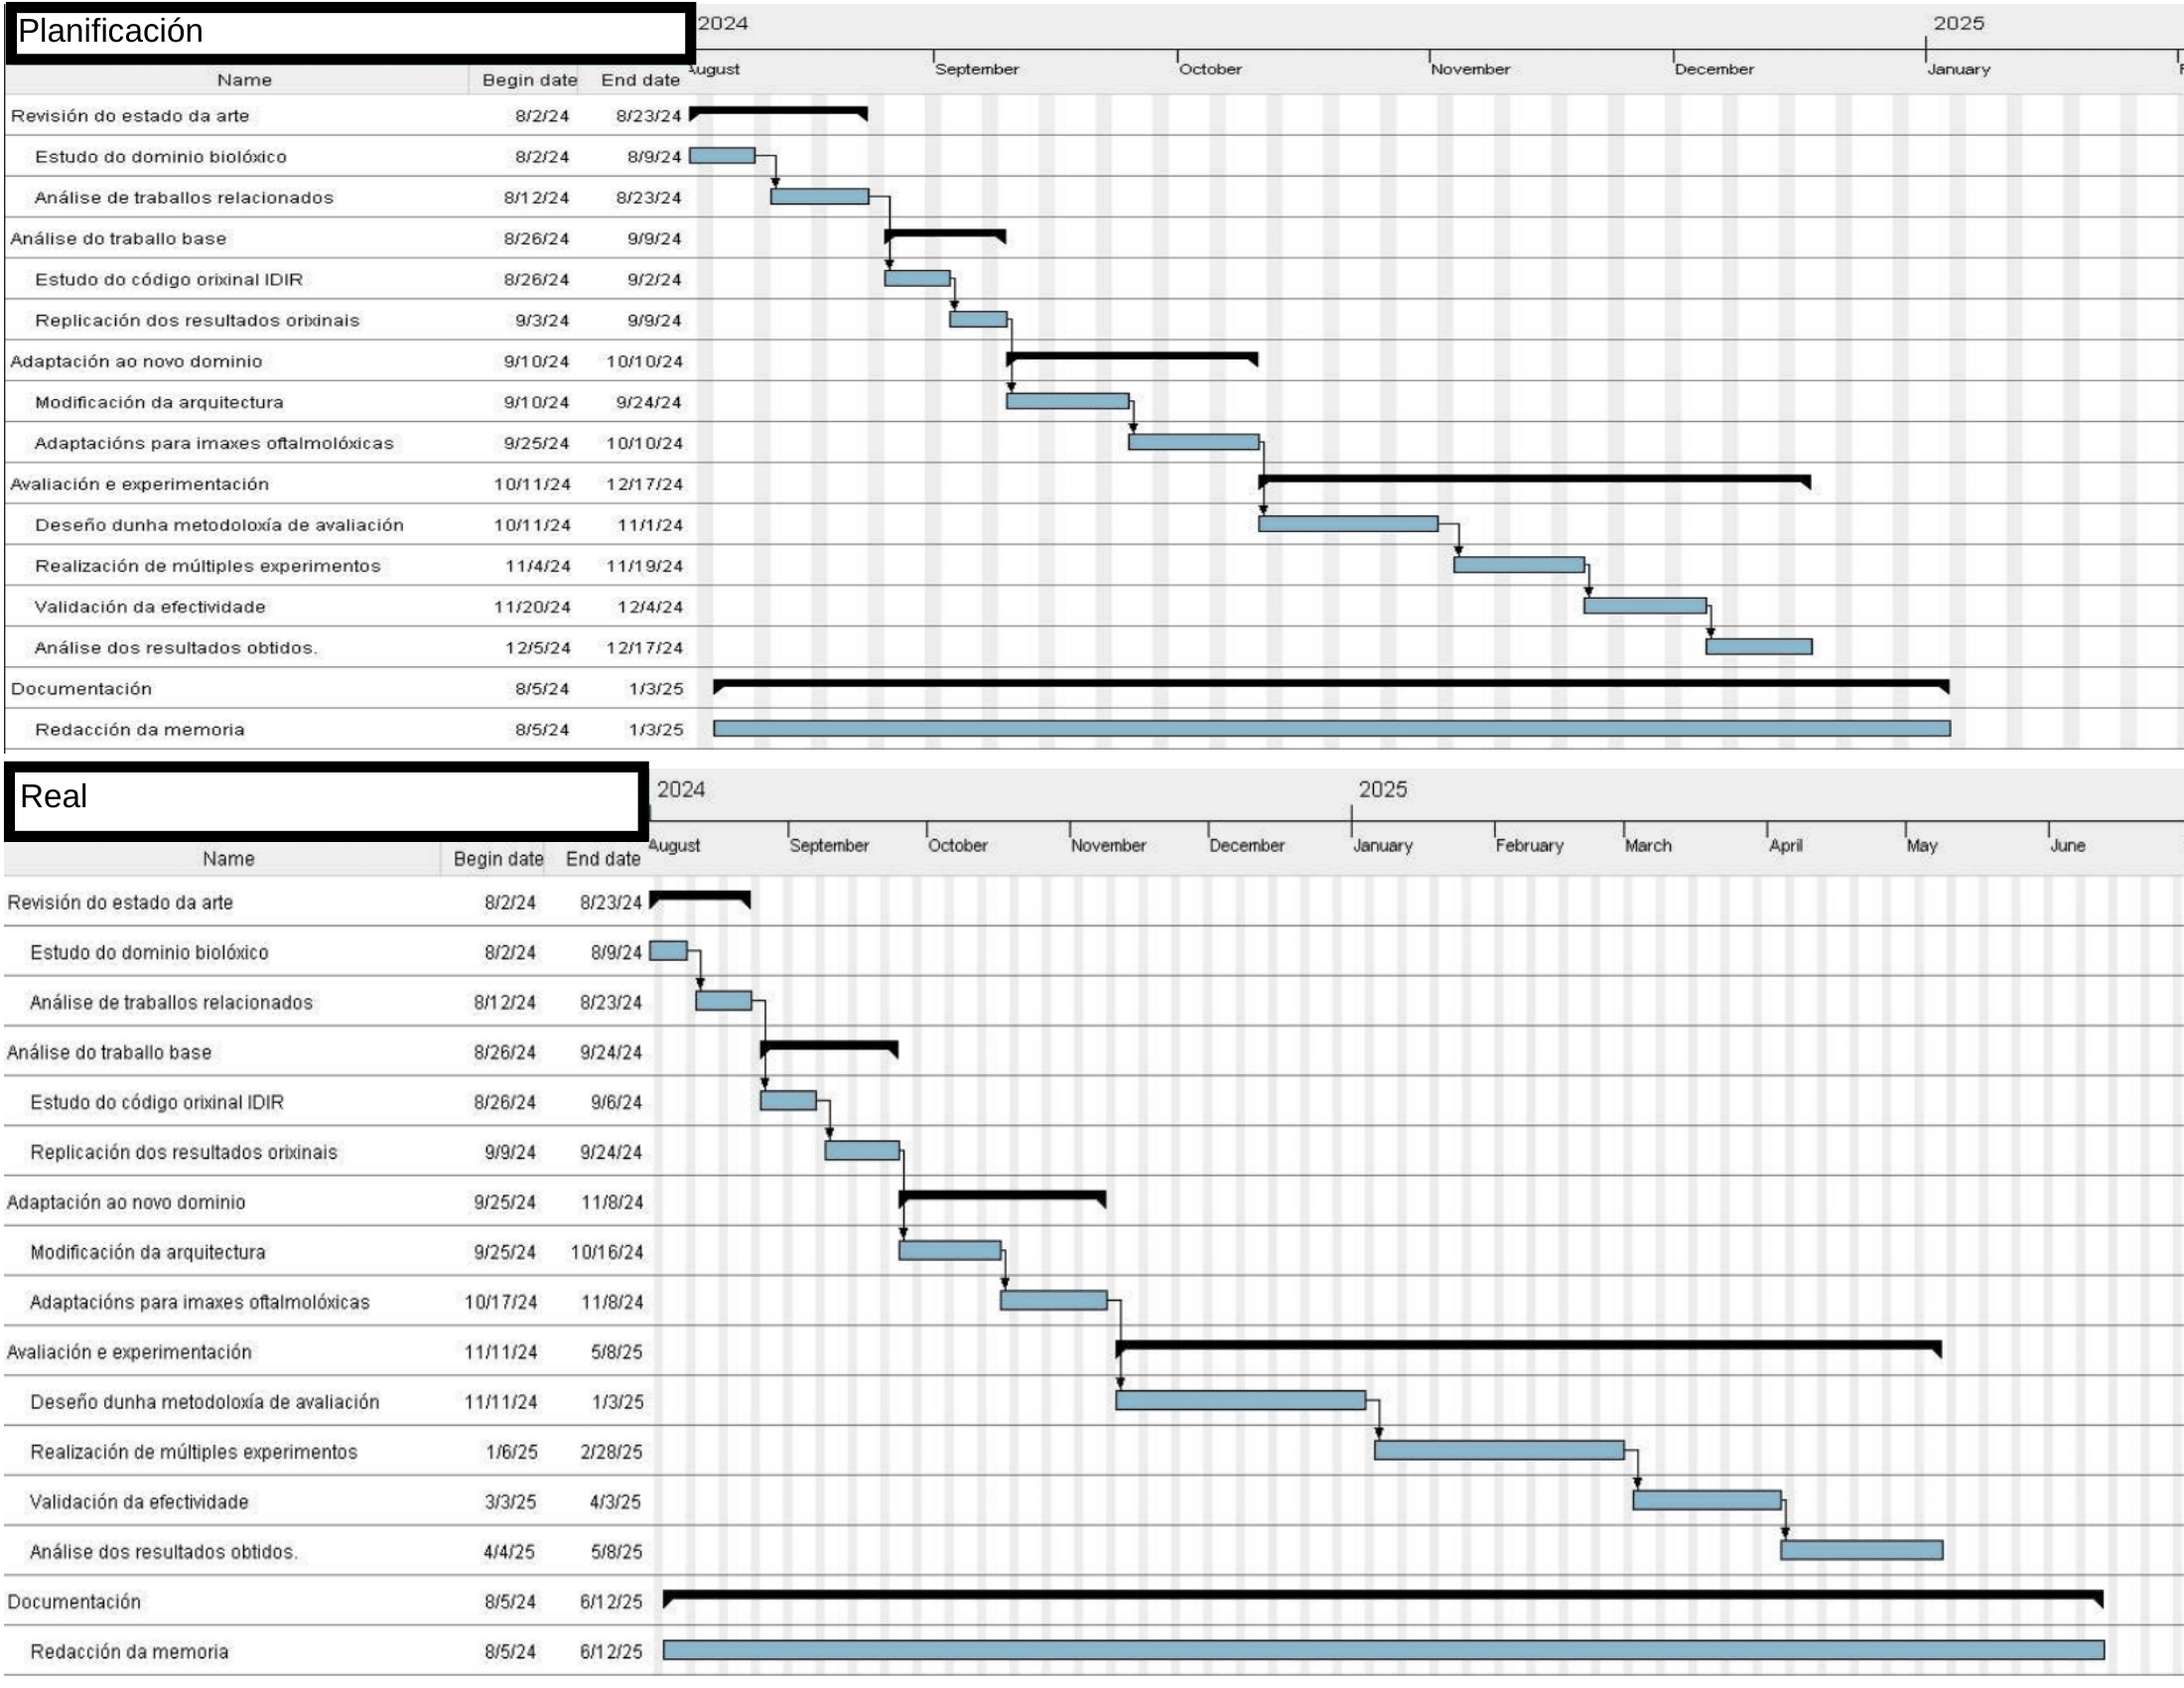
\includegraphics[height=1\textwidth, angle=90]{imaxes/gants-1.png}
    \caption{Diagramas de Gantt da planificación do proxecto e duración real de cada fase}
    \label{fig:planificacion_proxecto}
\end{figure}

\section{Recursos utilizados}
\label{sec:Recursos utilizados}

\subsection{Software}
\label{subsec:Software}

Xa que parte do traballo consiste en adaptar un traballo previo, 
decidíuse empregar moito do mesmo software ca o traballo orixinal para facilitar a implementación e reproducibilidade.
O mais relevante é PyTorch, unha librería de código aberto para Python que facilita o desenrolo de redes neuronais. Utilizáronse as versións de Python 3.12.3 e CUDA 12.2. Tamén se empregan librerías de apoio como NumPy (para traballar con matrices), Matplotlib (visualización), OpenCV ou scikit-learn (manexo de imaxes).

Outro software empregado inclúe VSCode (IDE), Git (control de versións) e LaTeX (redacción de memoria).

\subsection{Hardware}
\label{subsec:Hardware}

O proxecto foi desenrrolado nun ordenador portátil conectado por ssh a un servidor con GPU. 
Utilizáronse dous servidores diferentes, un montado por min\footnote{\url{https://blog.m19182.dev/writings/Building-my-Homelab}} e outro facilitado polo grupo de investigación VARPA (Visión Artificial y Reconocimiento de Patrones).

A gran parte dos experimentos foron realizado no primeiro, mais para poder executar o proxecto cas imaxes na súa resolución orixinal foi necesario empregar o segundo 
debido ás limitacións de memoria da GPU. Na táboa \ref{tab:comparativa_servidores} móstrase unha comparativa entre os servidores utilizados, indicando as principais características de hardware de cada un.

\begin{table}[tbp]
\centering
\begin{tabular}{|c|c|c|}
\hline
\textbf{Característica} & \textbf{Homelab} & \textbf{Servidor VARPA} \\ \hline
Procesador & AMD Ryzen 9 5950X&  AMD Ryzen Threadripper 3960X \\ \hline
GPU & NVIDIA RTX 3090 & NVIDIA RTX A6000  \\ \hline
\end{tabular}
\caption{Comparativa entre os servidores utilizados}
\label{tab:comparativa_servidores}
\end{table}


\subsection{Conxuntos de datos}
\label{subsec:Conxuntos de datos}
Para o desenrolo do proxecto empregáronse dous conxuntos de datos diferentes:

\begin{itemize}
    \item \textbf{RFMID:} 3200 imaxes de fondo de ollo en cor con resolución 1712x1712.
    \item \textbf{FIRE:} 134 pares de imaxes de retinas en cor, cun tamaño de 2912×2912 pixels
\end{itemize}

Estos son descritos en maior detalle na sección \ref{sec:Conxuntos de datos}.

\subsection{Estimación de custos}
\label{subsec:Estimación de custos}

Os custos do hardware son ignorados xa que xa estaba dispoñible antes da realización do proxecto.

Os custos dos recursos humanos calcúlanse para un estudante e dous titores, resultando nun custo estimado de 20.680€, IVE incluído. A táboa \ref{tab:estimacion_custos} mostra a estimación de custos dos recursos humanos desglosados, considerando un estudante a 20€/hora e titores a 35€/hora.

\begin{table}[h]
\centering
\begin{tabular}{|c|c|c|c|}
\hline
\textbf{Recurso} & \textbf{Custo por hora} & \textbf{Horas estimadas} & \textbf{Custo total} \\ \hline
Estudante & 20€ & 880h & 17.600€ \\ \hline
Titor 1 & 35€ & 44h & 1.540€ \\ \hline
Titor 2 & 35€ & 44h & 1.540€ \\ \hline
\end{tabular}
\caption{Estimación de custos dos recursos humanos (IVE incluído)}
\label{tab:estimacion_custos}
\end{table}

\section{Seguimento da planificación}
\label{sec:Seguimento da planificación}

A planificación do proxecto foi revisada periodicamente segundo as fases do proxecto, e para identificar desviacións respecto ao plan inicial.

Pese a que nas fases iniciais do proxecto se respectou a planificación, a fase de adaptación ao novo dominio e a fase de avaliación e experimentación sufriron retrasos significativos.

A fase de adaptación ao novo dominio requiriu máis tempo do esperado debido á complexidade das modificacións necesarias para adaptar o modelo a imaxes 2D, así como á necesidade de realizar múltiples probas para garantir o correcto funcionamento do modelo adaptado. A fase de avaliación tamén se viu afectada, xa que requiriu máis tempo do esperado para deseñar unha metodoloxía de avaliación adecuada. Finalmente, a fase de experimentación requiriu máis tempo do previsto, en parte debido aos malos resultados obtidos inicialmente, que obrigaron a revisar en profundidade o código e implementar novas probas para asegurar a correcta implementación.
En total, isto conlevou un retraso de aproximadamente 18 semanas respecto á planificación inicial.

A fase final de análise de resultados e redacción da memoria tamén se viu afectada, aínda que en menor medida, o que conlevou un retraso adicional de 2 semanas, resultando nunha duración total do proxecto de 40 semanas, fronte ás 20 semanas inicialmente previstas.

Na figura \ref{fig:planificacion_proxecto} móstrase o diagrama de Gantt actualizado, que reflicte a duración real de cada fase do proxecto.

\subsection{Estimación de custo real}
\label{subsec:Estimación de custo real}

A estimación de custo do proxecto foi de 20.680€, como se indicou na sección \ref{subsec:Estimación de custos}. Non obstante, debido aos retrasos no desenvolvemento do proxecto, o custo real aumentou de forma proporcional ao tempo extra empregado.

Dado que o proxecto se estendeu durante 20 semanas máis do previsto (o dobre da planificación inicial), o custo real estimado ascende a 41.360€ (IVE incluído).
 \chapter{Experimentos e resultados}
\label{chap:Experimentos e resultados}
\lettrine{N}{este} capítulo presentaranse os experimentos realizados e os resultados obtidos.
Para iso, comezarase presentando unha vista xeral do proceso de experimentación, incluída a avaliación, así como os conxuntos de datos empregados.
A continuación, presentaranse os resultados obtidos cas diferentes configuracións probadas.

\section{Vista Xeral}
\label{sec:Vista Xeral}

\section{Conxuntos de datos}
\label{sec:Conxuntos de datos}

\subsection{FIRE}
\label{subsec:FIRE}

\subsection{RFMID}
\label{subsec:RFMID}

\section{Avaliación}
\label{sec:Avaliación}
  \chapter{Traballo Realizado}
\label{chap:Traballo Realizado}

\lettrine{N}{este} apartado presentarase o traballo realizado, comezando por unha vista xeral do proceso, 
seguido dunha explicación dos diferentes módulos desenvolvidos e a súa interacción.
Finalmete, presentaranse os resultados obtidos acompañados dunha análise dos mesmos.
\section{Vista Xeral}
\label{sec:Vista Xeral}


\section{Discusión}
\label{sec:Discusión}
  \chapter{Conclusións}
\label{chap:Conclusións}

\lettrine{E}{n} conclusión, o proxecto de investigación realizado consistiu na adaptación do framework IDIR para o rexistro de retinografías.
En especial valoramos o uso da función de activación SIREN, proposta como alternativa á función ReLU para mellorar a representación das deformacións.

A aliñación de retinografías é un problema relevante xa que é un proceso laborioso para os expertos, mais con moita uilidade clínica.
A etapa inicial da revisión do estado da arte revelou que xa existían varios traballos previos que abordaban este problema, sendo os máis exitosos os baseados en métodos iterativos.
Actualmente os métodos de aprendizaxe profunda son unha alternativa prometedora que está gañando prominencia no campo. Particularmente, o uso de representacións implícitas para esta tarefa é un enfoque innovador que xa foi aplicado en outros campos da imaxe médica con bós resultados.

Para avaliar a efectividade do método proposto, escolléronse dous conxuntos de datos de retinografías: FIRE, que permite a avaliación do método en imaxes reais, e RFMID, sobre o que se efectuaron transformacións artificiais para simular diferentes escenarios de aliñación.

Durante a fase de experimentación exploráronse diferentes combinacións de hiperparámetros (loss, regularización, resolución, batch size...) e introducíronse diferentes técnicas para tentar mellorar a converxencia do modelo, como diferentes esquemas de mostraxe, inicialización, e técnicas de axuste dinámico do batch size.

Algunhas das dificultades atopadas durante o desenrrolo do proxecto foron: a falta de documentación sobre o funcionamento do código orixinal, que dificultou a súa adaptación ao novo dominio; o deseño do proceso de avaliación, no cal foi complexo atopar visualizacións que permitisen interpretar os resultados facilmente; e o tempo de cómputo que requerían algúns experimentos, que requeriu a implementación de optimizacións para facilitar a experimentación.

Os resultados obtidos amosan que esta arquitectura non é a máis adecuada para a tarefa de rexistro de retinografías.

Si que se obteñen bós resultados no dataset RFMID, que se basea en imaxes con transformacións lineais sintéticas, onde a función de activación ReLU tende a obter mellores resultados ca SIREN, xa que está mellor preparada para representar as transformacións lineais globais que se producen entre estas imaxes.
Obsérvase tamén que o tamaño da transformación ten un impacto significativo no rendemento, xa que as imaxes de maior tamaño presentan un maior erro de rexistro.

No dataset FIRE, que contén imaxes reais, os resultados son peores ca no dataset RFMID, especialmente nas parellas de imaxes que presentan grandes deformacións ou baixo nivel de superposición.
A función de activación SIREN obtén mellores resultados aquí, xa que é capaz de representar mellor as deformacións non lineais e locais que se producen entre as imaxes.

Estas diferencias no rendemento destacan a importancia da elección da función de activación en función da natureza específica das transformacións esperadas.
A fase de experimentación tamén revelou que a regularización é un factor fundamental, especialmente na función de activación SIREN, onde a ausencia de regularización leva a un sobreaxuste significativo e a un rendemento moi pobre.

Cabe destacar que o método presentado neste traballo guía a optimización con tan só a métrica de NCC, que depende únicamente das intensidades dos píxeles, e que en rexitros con moito desprazamento ou deformacións complexas a topografía de función de perda será pouco convexa e con múltiples mínimos locais, o que dificulta a converxencia do modelo.
Polo contrario, métodos como REMPE \cite{rempe} que obteñen resultados moito mellores (rexistra exitosamente a totalidade da categoría S de FIRE) fan uso de información adicional que lles permite establecer correspondencias globais entre as imaxes.

Unha observación relevante é a diferencia entre o rendemento entre o conxunto de datos sintético (RFMID) e o conxunto de datos real (FIRE). Esta brecha demostra a dificultade de aplicar modelos adestrados en datos sintéticos a imaxes reais.

Todos estes achados responden aos obxectivos propostos no inicio do proxecto, onde adaptamos o framework IDIR para o rexistro de retinografías, exploramos a función de activación SIREN e avaliamos o rendemento do modelo en diferentes condicións.

  \chapter{Traballo futuro}
\label{chap:Traballo futuro}

\lettrine{E}{xisten} varias liñas de traballo futuro que se poden seguir para mellorar o sistema actual.
 Os resultados obtidos neste traballo, aínda que demostran a viabilidade de adaptar o framework IDIR para o aliñamento de imaxes oftalmolóxicas 2D, tamén revelan limitacións á hora de acadar a precisión e robustez desexables.
 As seguintes liñas de traballo futuro considéranse prometedoras para superar estes desafíos e avanzar no campo:

% \section{Instant Neural Graphics Primitives}
% \label{sec:Instant Neural Graphics Primitives}

% Introducidas por \cite{mueller2022instant}, propoñen encodear os inputs da rede a un espacio dimensional superior.

% Encodear os inputs da rede é unha técnica que xa se emprega en moitas ocasións (one-hot encodings, transformers...)
% Eles utilizan 'sparse parametric encodings' utilizando unha tabla de hashes de múltiples resolucións, que tamén tén parámetros entrenables e fai parte do traballo de aprendizaxe da rede.
% Isto permítelles un entrenamento e inferencia moito mais rápido que outros métodos, sen ter que sacrificar en rendemento.

% \cite{li2024neuralgraphicsprimitivesdeformable} aplicao estas ideas á tarefa de rexistro, con moi bós resultados.
% Notablemente, resuelven o 'sliding boundary problem', que se refiere ás complicación de modelar o movemento relativo entre diferentes estructuras. 
% No caso da imaxe pulmonar, surxe cuando os lóbulos dos pulmóns se deslizan entre sí durante la respiración.

\section{Arquitecturas alternativas}
\label{sec:Arquitecturas alternativas}

Unha liña relevante de traballo futuro é a exploración de arquitecturas alternativas. 
Mentres que os perceptróns multicapa (MLPs) son considerados aproximadores universais \cite{HORNIK1989359} (son capaces de aproximar calquera función continua dada unha cantidade suficiente de neuronas), é posible que a arquitectura utilizada de 3 capas con 256 neuronas por capa non sexa o suficientemente grande para capturar as complexidades das transformacións entre as retinografías.

Unha opción sería aumentar o número de capas ou neuronas por capa. Outra sería implementar o use de codificación posicional, que parece ser útil para a tarefa de rexistro \cite{mueller2022instant}.

Outra idea moi intersante é o use de restriccóns de consistencia cíclicas, propostas por Van Harten et al. no contexto de rexistro de imaxes médicas \cite{van_Harten_2024}. Consiste en entrenar dúas redes á vez que estiman as transformacións directas e inversas, facendo que estas se regularicen mutuamente e estabilizando a optimización.

\section{Invertibilidade}
\label{sec:Invertibilidade}

Unha direción interesante para o traballo futuro é a exploración de métodos que garantan a invertibilidade das transformacións aprendidas pola rede.
A rede IDIR actual non garante a invertibilidade das transformacións aprendidas, o que significa que non é posíbel aplicar a transformación inversa de maneira fiable.

Grazas aos termos de regularización utilizados durante o adestramento son poucos os casos nos que o determinante jacobiano é negativo (o que indicaría que a transformación non é invertible).

Aproximación como a de i-RevNet \cite{jacobsen2018irevnetdeepinvertiblenetworks} ou aqueles baseados en campos vectoriais de velocidade \cite{sun2024medicalimageregistrationneural} permiten garantir a invertibilidade das transformacións aprendidas, o que podería mellorar a precisión e a robustez do rexistro e funcionaría como un mecanismo de regulación implícita.

\section{Enfoque híbrido}
\label{sec:Enfoque híbrido}

Outra liña de traballo futuro é a exploración de enfoques híbridos que combinen o rexistro baseado en redes neuronais con técnicas tradicionais de rexistro.
Unha posibilidade sería utilizar o rexistro tradicional para proporcionar un rexistro inicial robusto, que despois podería ser refinado por unha rede neuronal.

Así mesmo, poderíanse explorar con máis profundidade o preprocesado das imaxes, xa que é inexistente no método actual pero podería ser útil para mellorar a calidade das imaxes e facilitar o rexistro.

 %%%%%%%%%%%%%%%%%%%%%%%%%%%%%%%%%%%%%%%%
 % Apéndices, glosarios e bibliografía  %
 %%%%%%%%%%%%%%%%%%%%%%%%%%%%%%%%%%%%%%%%

 \appendix
 \appendixpage
%  \chapter{Material adicional}
\label{chap:adicional}

\section{Anexo regularization}
\label{sec:Anexo regularization}

% \begin{table}[h]
%     \centering
%     \begin{minipage}[t]{0.45\linewidth}
%         \centering
%         \scriptsize
%         \setlength{\tabcolsep}{25pt}
%         \begin{tabular}{|c|c|}
%         \hline
%         Resolution & Mean Distance \\ \hline
%         100 & 254.22 \\ \hline
%         250 & 251.29 \\ \hline
%         750 & 250.62 \\ \hline
%         1250 & 250.59 \\ \hline
%         1708 & 249.72 \\ \hline
%         \end{tabular}
%         \caption{Distancias medias para o dataset FIRE ca función de activación Relu}
%         \label{tab:mlp_mean_distances_fire}
%     \end{minipage}
%     \hfill
%     \begin{minipage}[t]{0.45\linewidth}
%         \centering
%         \scriptsize
%         \setlength{\tabcolsep}{25pt}
%         \begin{tabular}{|c|c|}
%         \hline
%         Resolution & Mean Distance \\ \hline
%         100 & 266.43 \\ \hline
%         250 & 263.85 \\ \hline
%         750 & 263.19 \\ \hline
%         1250 & 258.56 \\ \hline
%         1708 & 258.06 \\ \hline
%         \end{tabular}
%         \caption{Distancias medias para o dataset FIRE ca función de activación SIREN}
%         \label{tab:siren_mean_distances_fire}
%     \end{minipage}
% \end{table}

% \begin{table}[h]
%     \centering
%     \begin{minipage}[t]{0.45\linewidth}
%         \centering
%         \scriptsize
%         \setlength{\tabcolsep}{25pt}
%         \begin{tabular}{|c|c|}
%         \hline
%         Resolution & Mean Distance \\ \hline
%         100 & 37.29 \\ \hline
%         250 & 36.18 \\ \hline
%         750 & 36.01 \\ \hline
%         1250 & 35.03 \\ \hline
%         1708 & 35.04 \\ \hline
%         \end{tabular}
%         \caption{Distancias medias para o dataset RFMID ca función de activación Relu}
%         \label{tab:mlp_mean_distances_rfmid}
%     \end{minipage}
%     \hfill
%     \begin{minipage}[t]{0.45\linewidth}
%         \centering
%         \scriptsize
%         \setlength{\tabcolsep}{25pt}
%         \begin{tabular}{|c|c|}
%         \hline
%         Resolution & Mean Distance \\ \hline
%         100 & 68.12 \\ \hline
%         250 & 73.42 \\ \hline
%         750 & 77.55 \\ \hline
%         1250 & 67.33 \\ \hline
%         1708 & 67.31 \\ \hline
%         \end{tabular}
%         \caption{Distancias medias para o dataset RMIFD ca función de activación SIREN}
%         \label{tab:siren_mean_distances_rfmid}
%     \end{minipage}
% \end{table}


\subsection{Figuras experimentos de regularización}
\label{subsec:figuras_experimentos_regularizacion}

\paragraph{Resultados}
\label{par:Resultados-reg2}

Os resultados da experimentación extendida da regularización, realizados sobre os datasets FIRE e RFMID, preséntanse nas figuras \ref{fig:gs_single_heatmaps}.

\begin{figure}[tbp]
    \centering
    \begin{subfigure}[b]{0.4\textwidth}
        \centering
        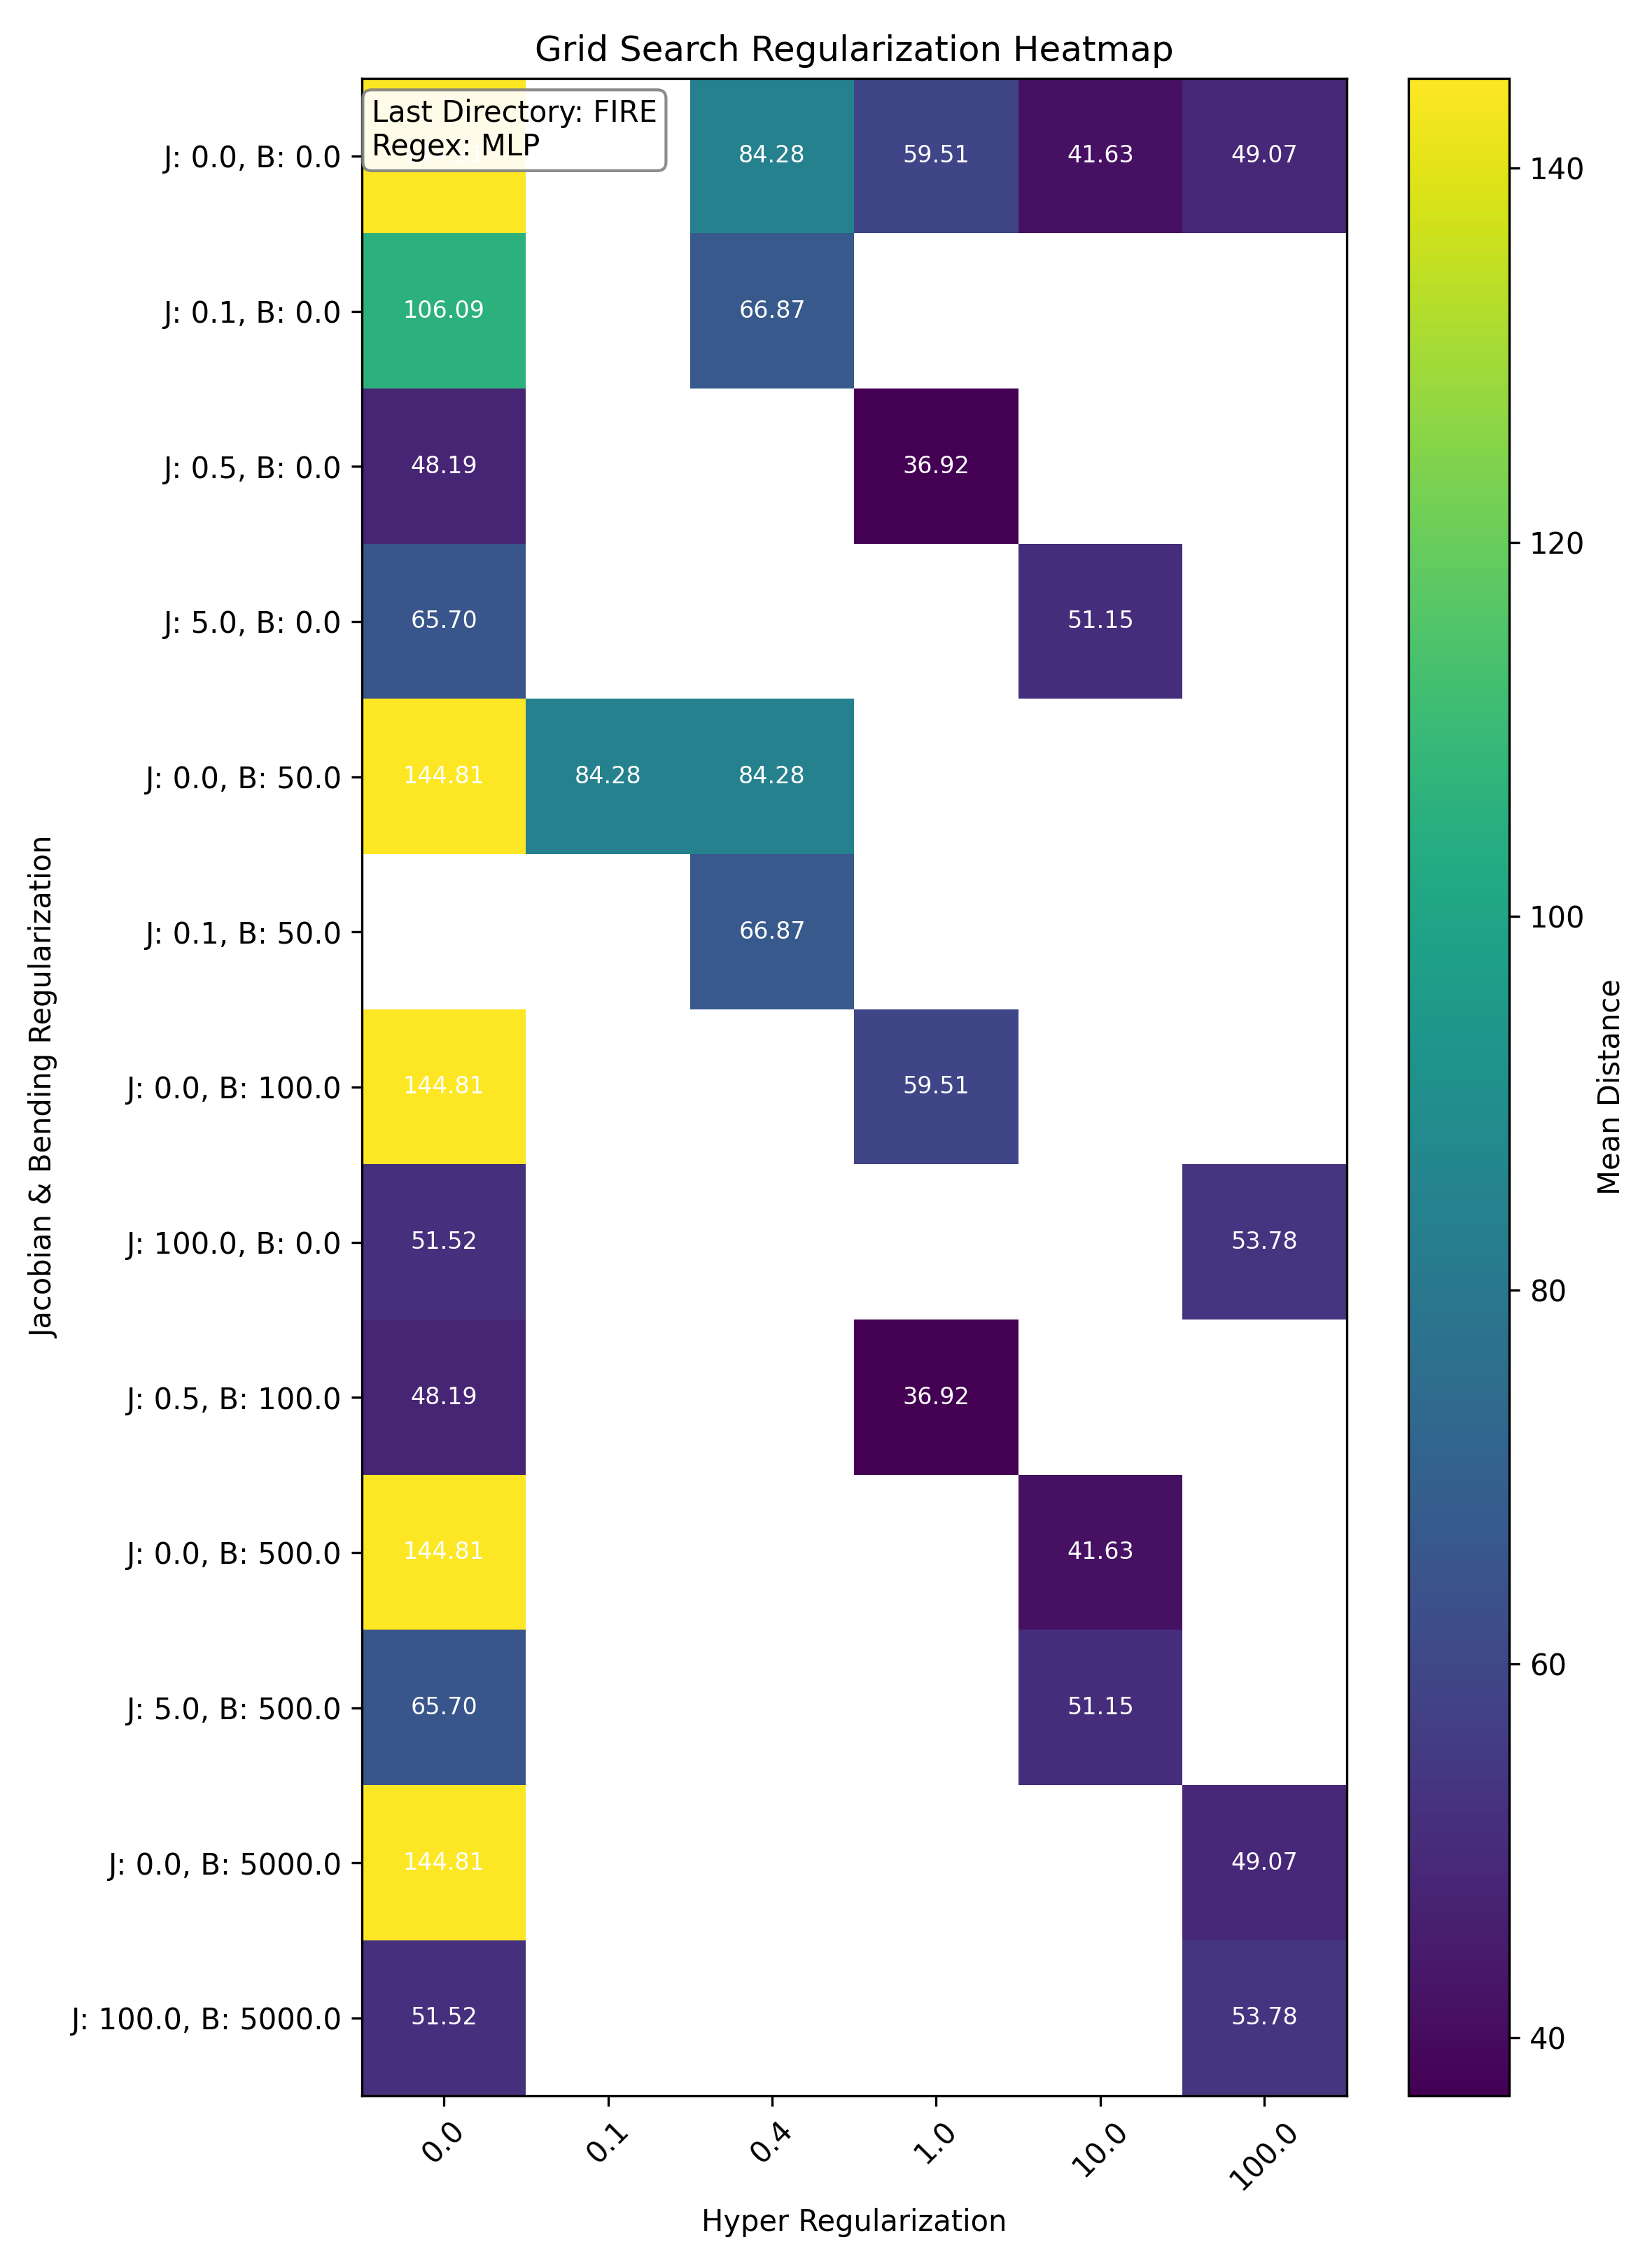
\includegraphics[width=\textwidth]{imaxes/grid_search_single_heatmap_FIRE_MLP.png}
        \caption{FIRE - Relu}
        \label{fig:gs_single_FIRE_MLP}
    \end{subfigure}\hfill
    \begin{subfigure}[b]{0.4\textwidth}
        \centering
        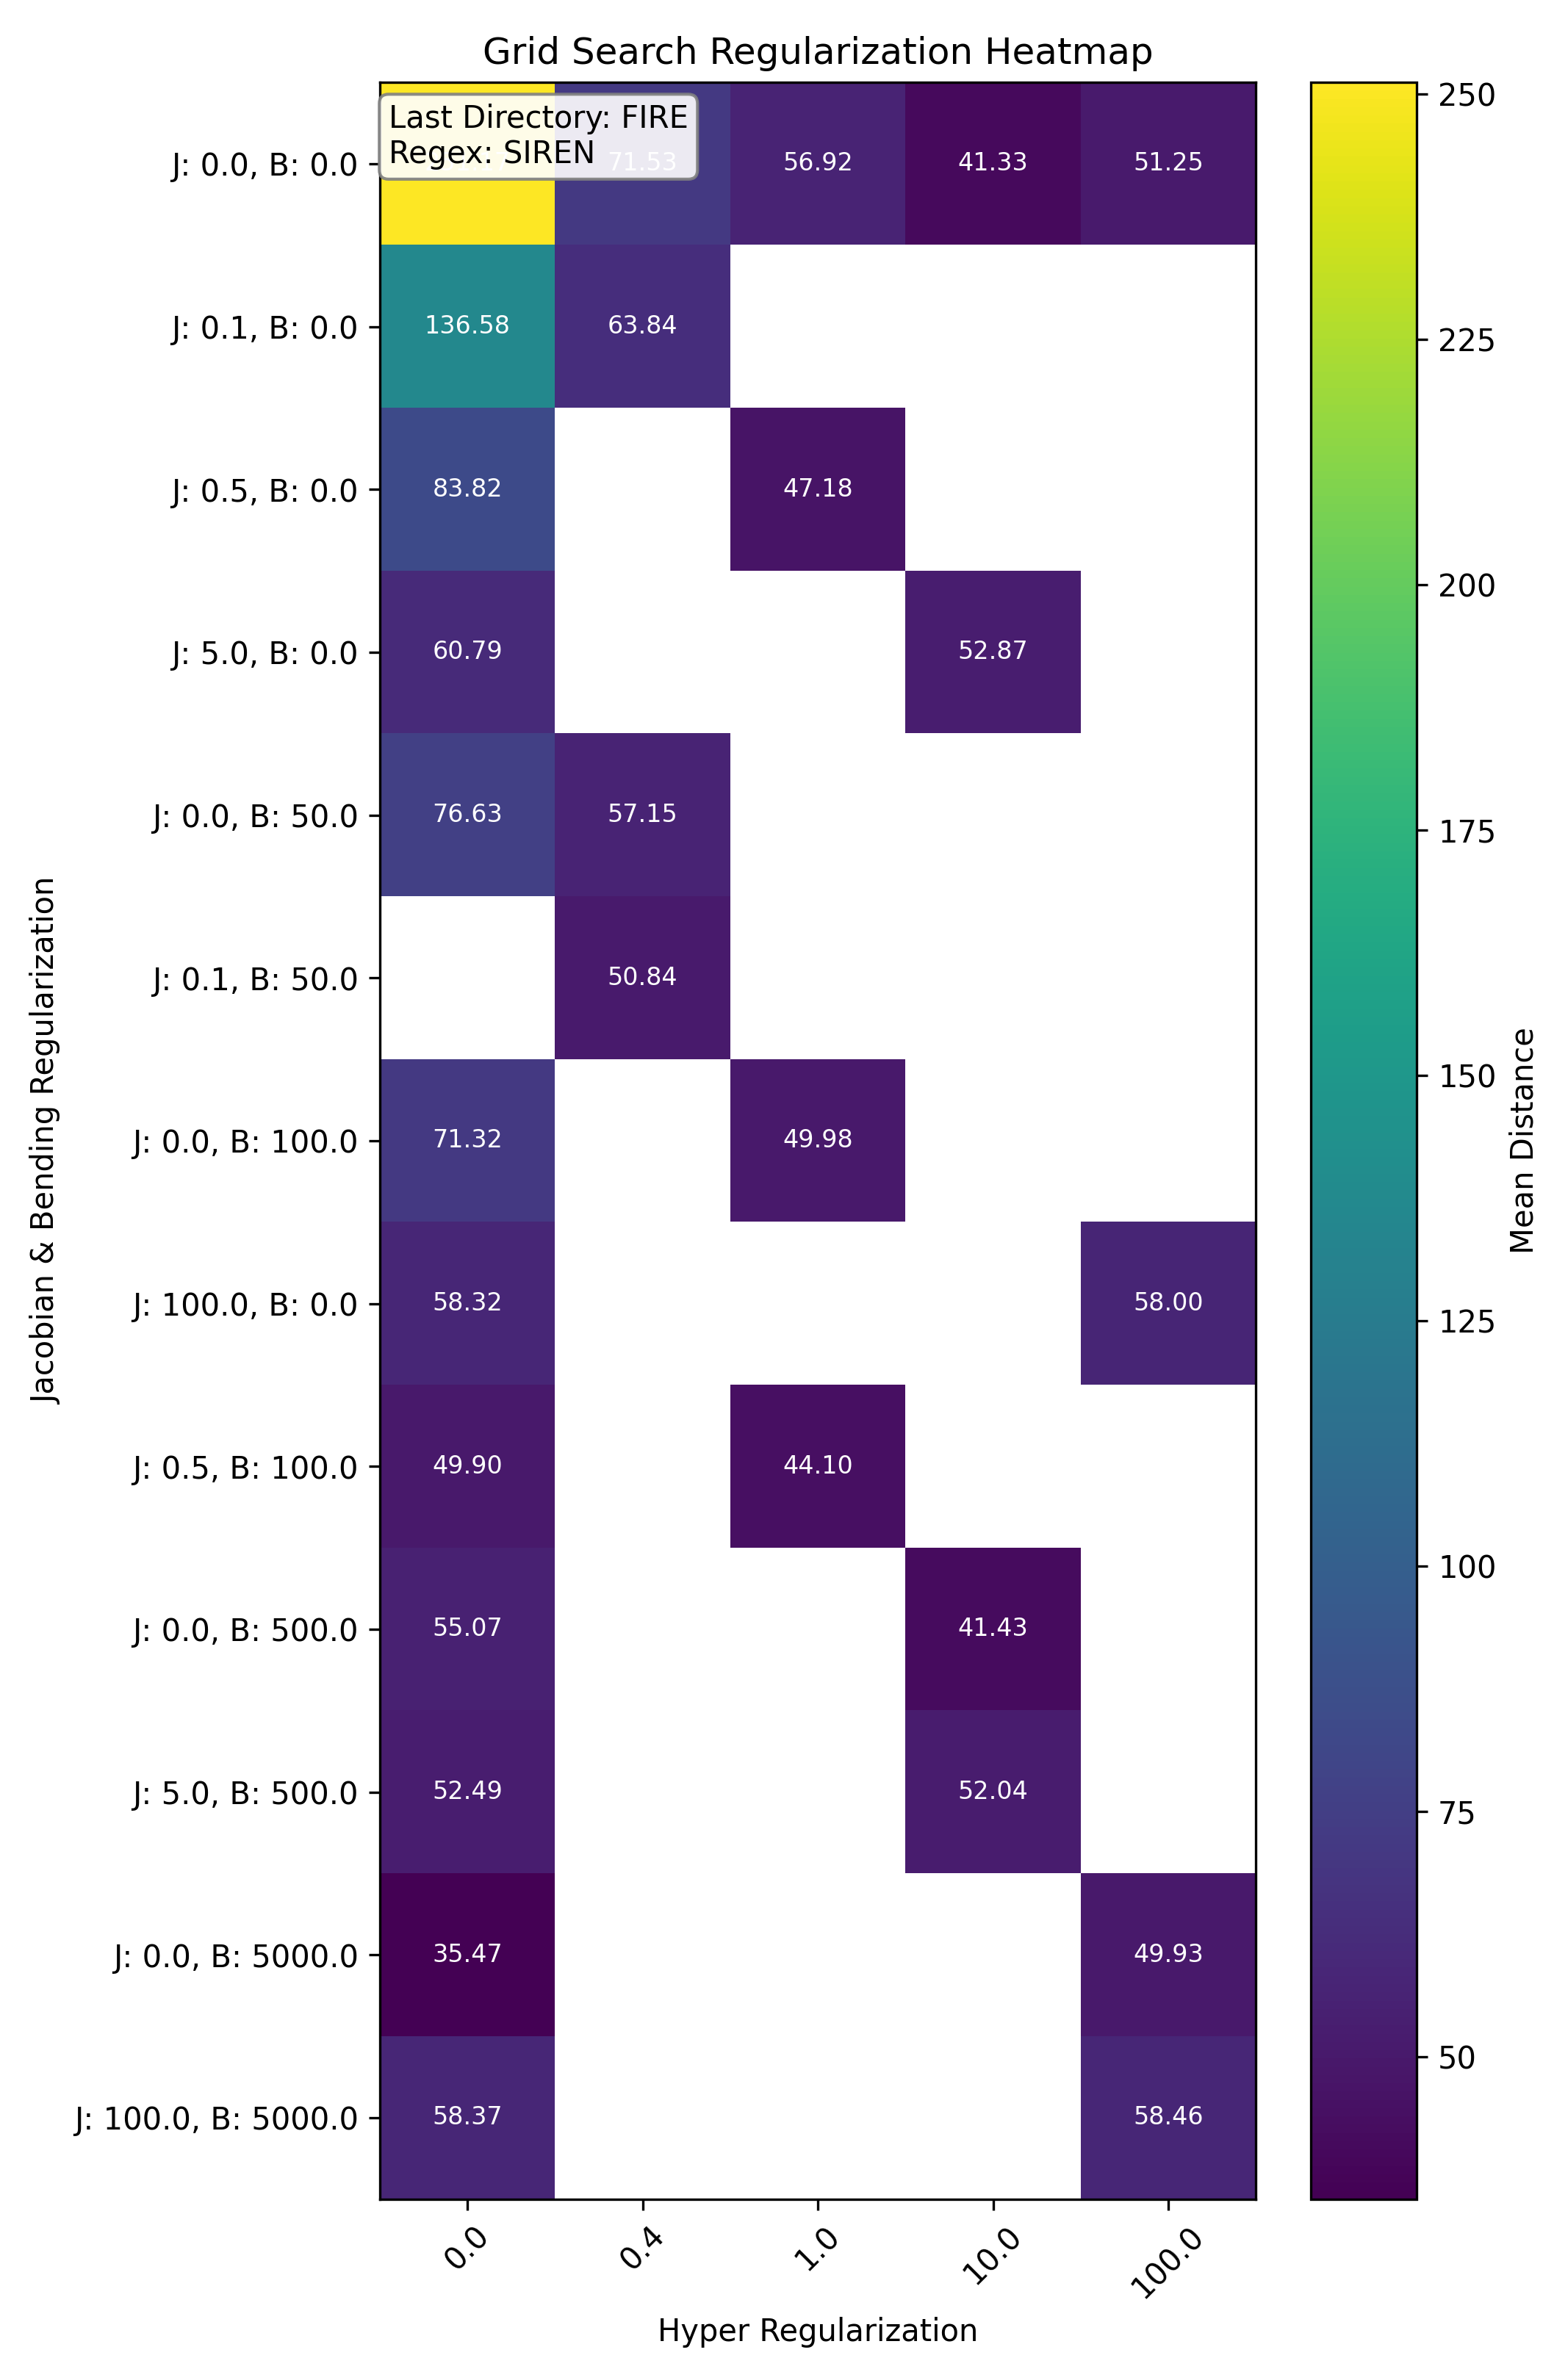
\includegraphics[width=\textwidth]{imaxes/grid_search_single_heatmap_FIRE_SIREN.png}
        \caption{FIRE - SIREN}
        \label{fig:gs_single_FIRE_SIREN}
    \end{subfigure}
    
    \vskip0\baselineskip
    
    \begin{subfigure}[b]{0.4\textwidth}
        \centering
        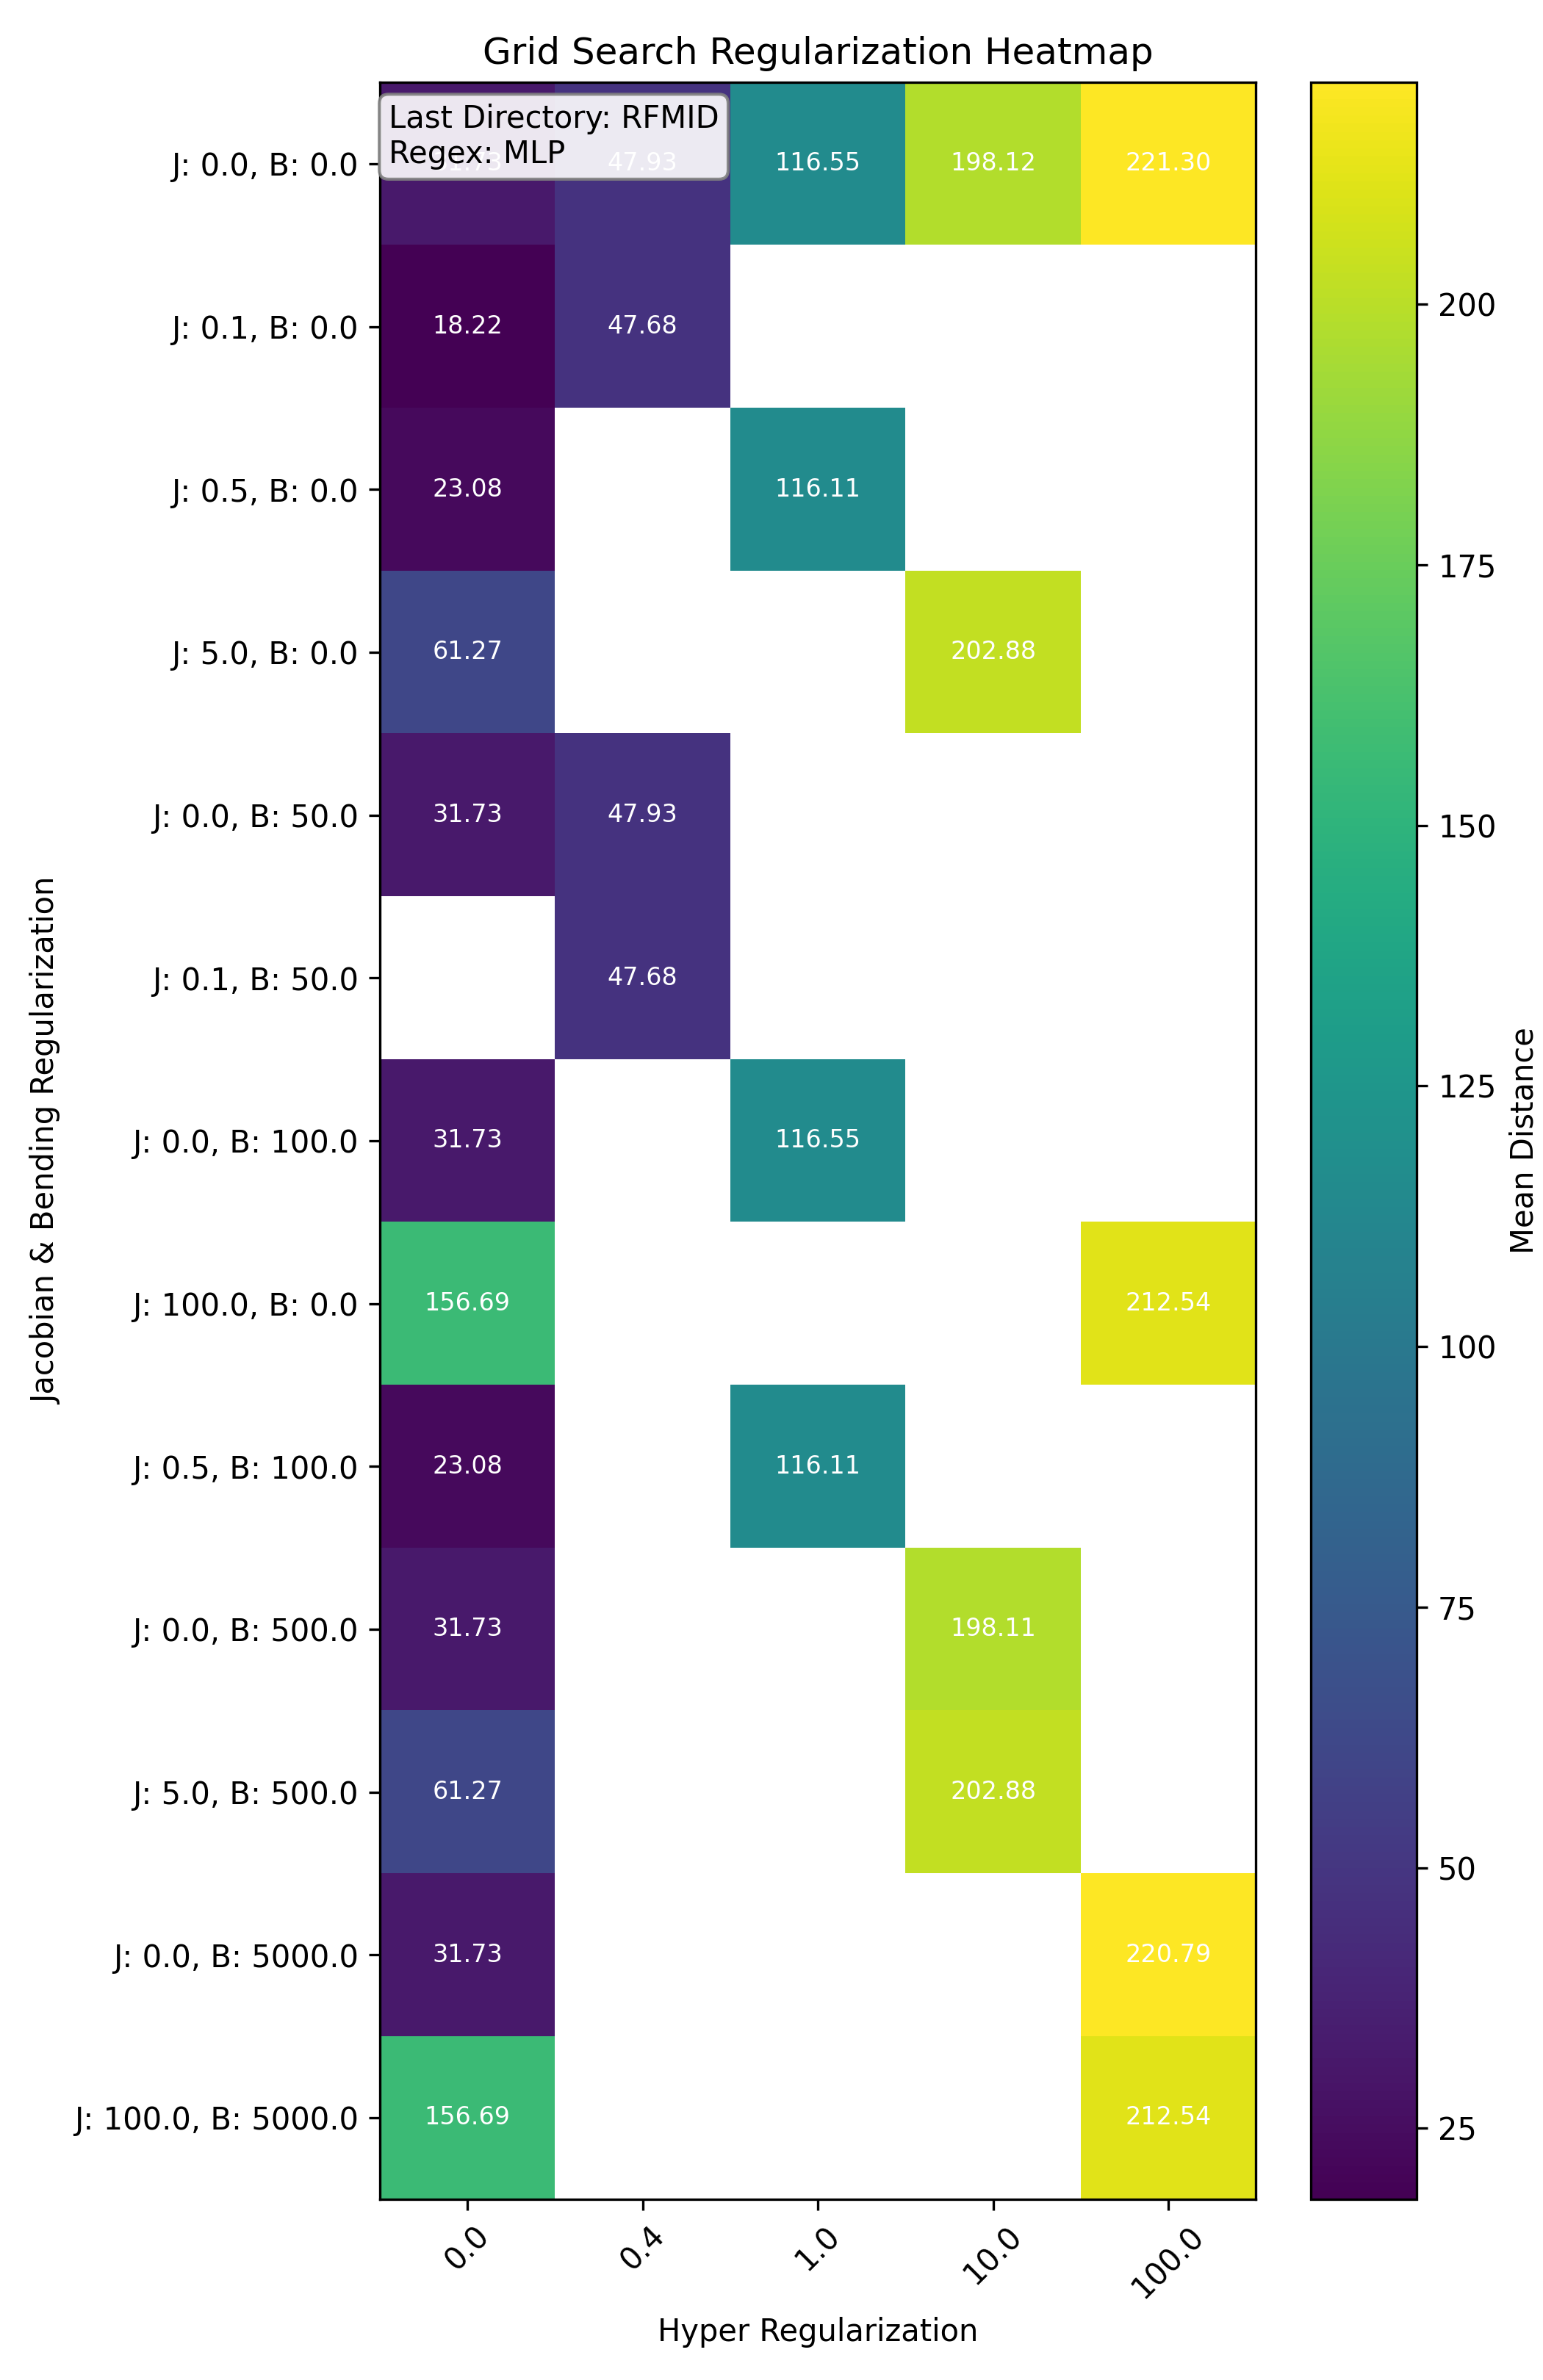
\includegraphics[width=\textwidth]{imaxes/grid_search_single_heatmap_RFMID_MLP.png}
        \caption{RFMID - Relu}
        \label{fig:gs_single_RFMID_MLP}
    \end{subfigure}\hfill
    \begin{subfigure}[b]{0.4\textwidth}
        \centering
        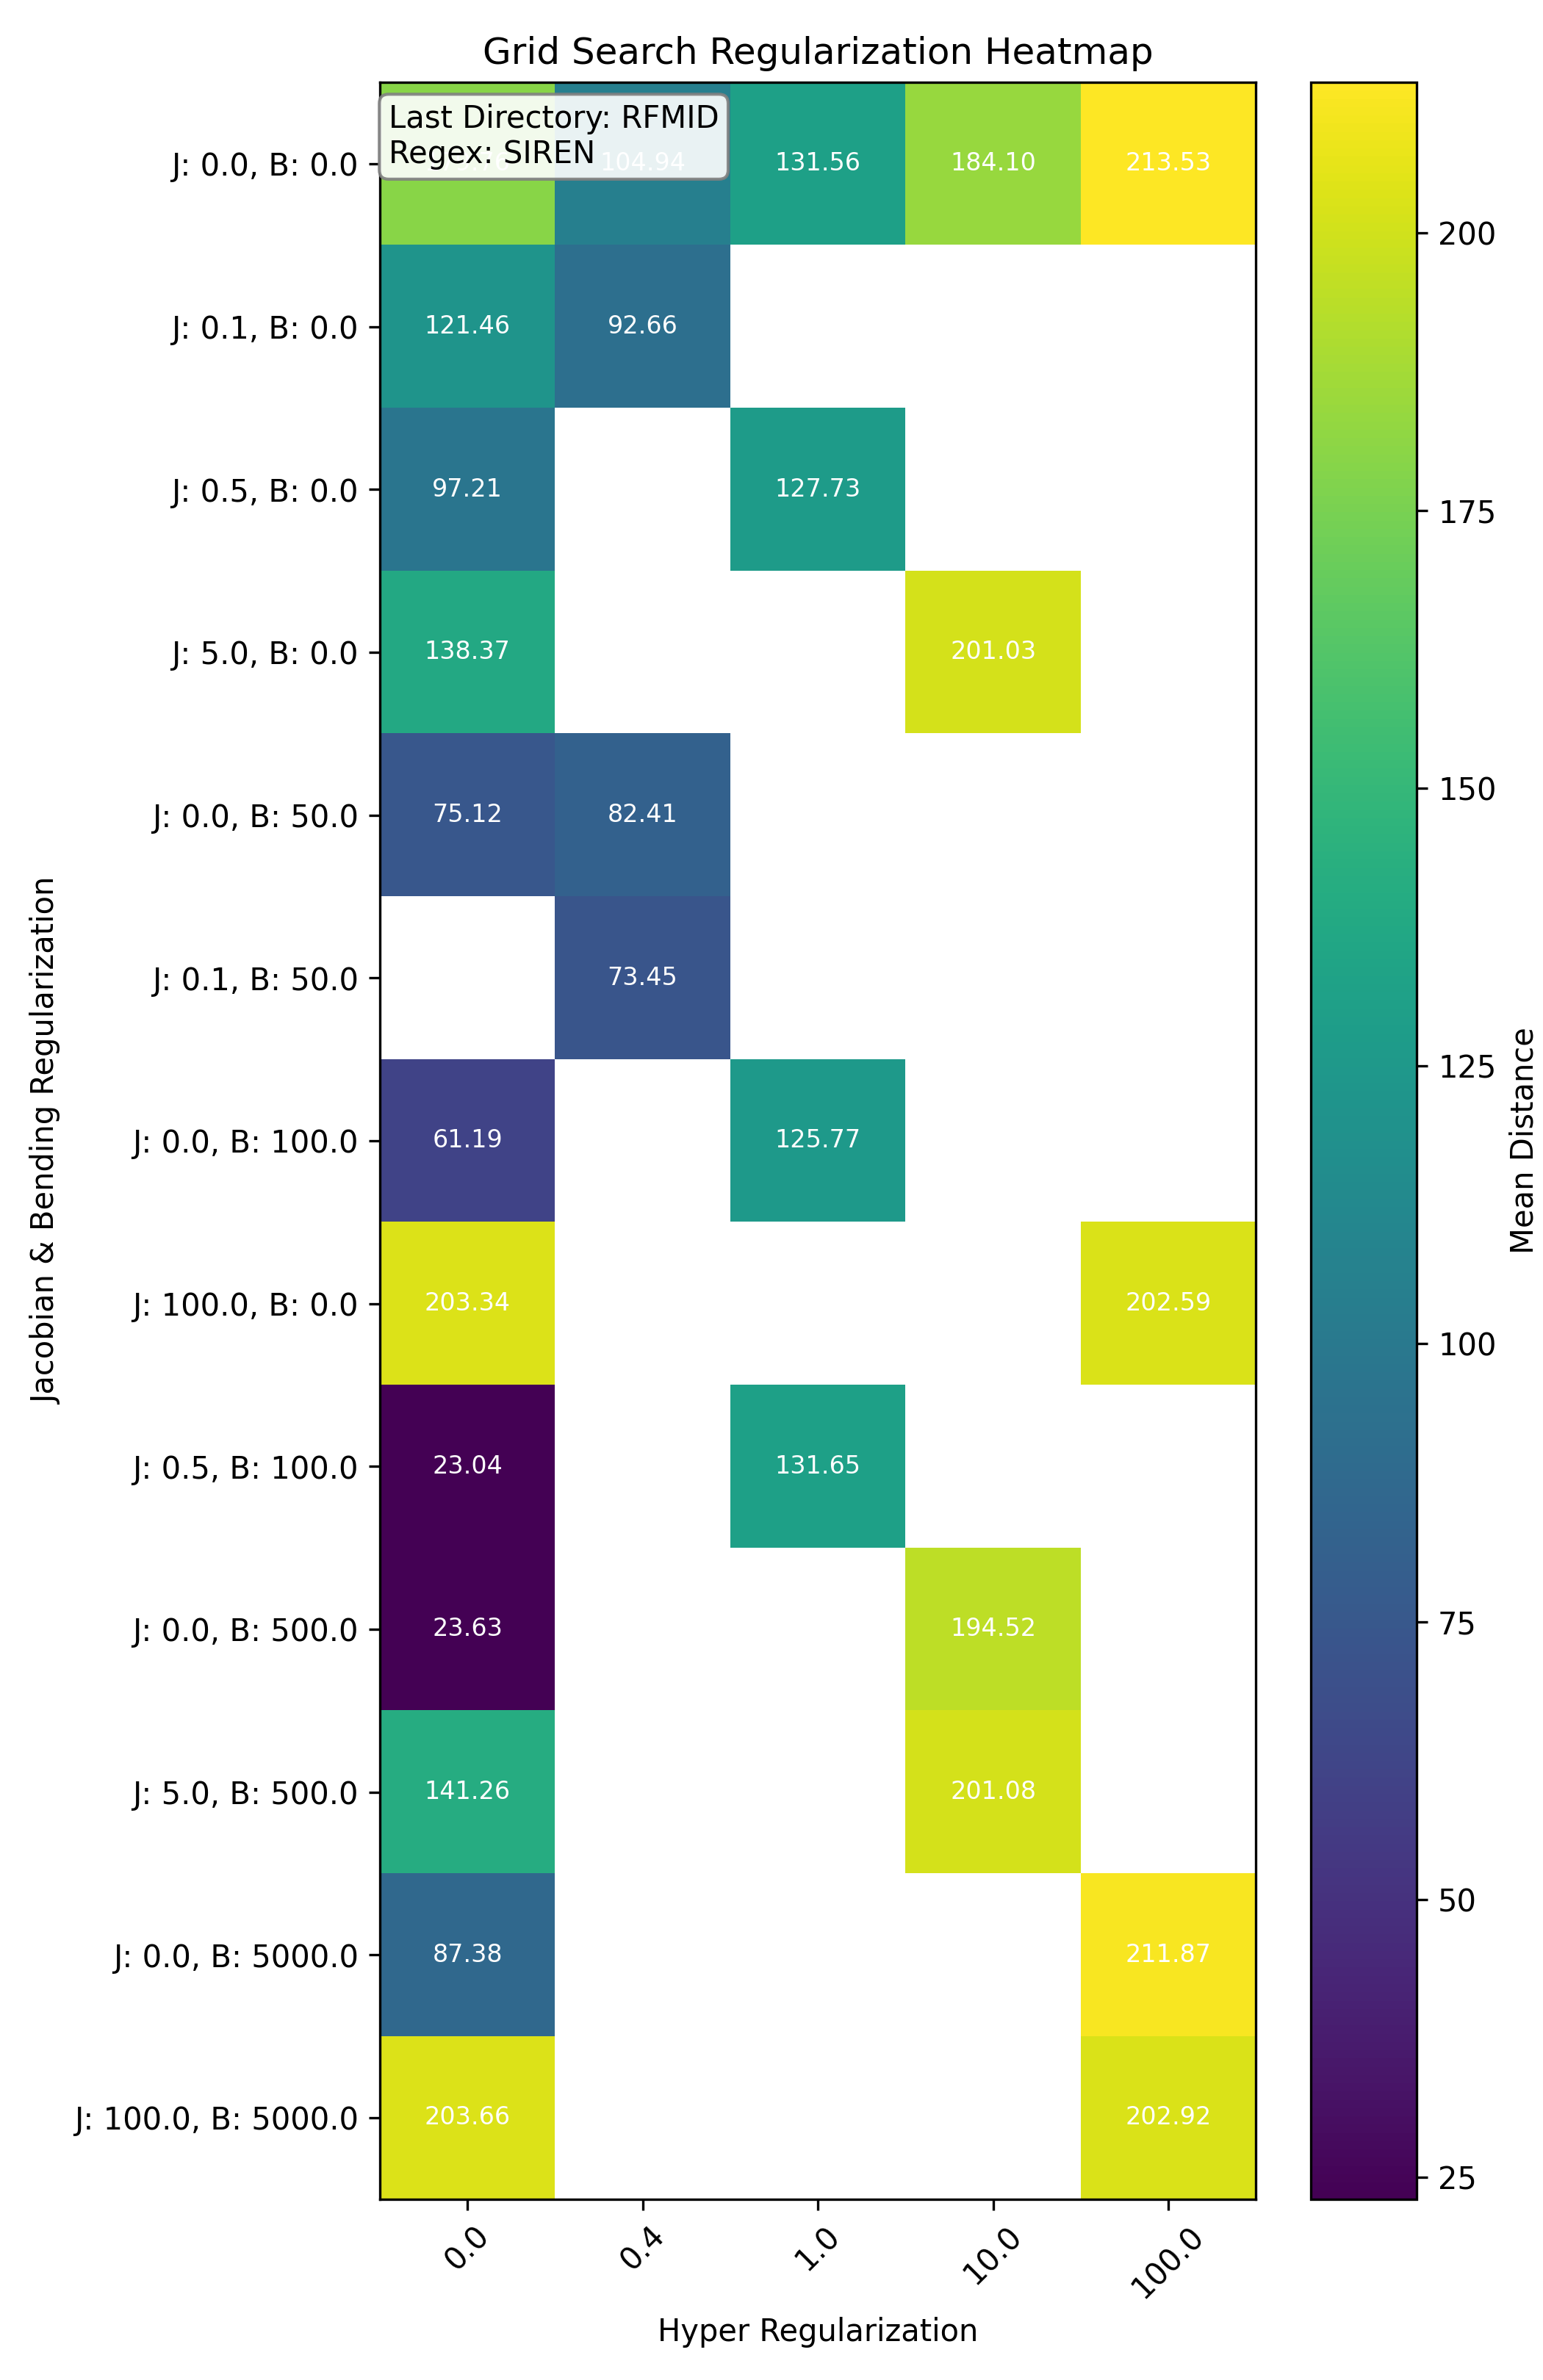
\includegraphics[width=\textwidth]{imaxes/grid_search_single_heatmap_RFMID_SIREN.png}
        \caption{RFMID - SIREN}
        \label{fig:gs_single_RFMID_SIREN}
    \end{subfigure}
    
    \caption{Mapa de calor cos resultados de diferentes combinacións de termos de regularización e funcións de activación sobre os datasets FIRE e RFMID}
    \label{fig:gs_single_heatmaps}
\end{figure}

\paragraph{Discusión}
\label{par:Discusion-reg2}

Os resultados amosan que as interaccións entre os diferentes termos de regularización e as funcións de activación son complexas e moi dependentes da parella de imaxes concreta a rexistrar.

\FloatBarrier
%\include{anexos/...}

 \printglossary[type=\acronymtype,title=\nomeglosarioacronimos]
 \printglossary[title=\nomeglosariotermos]

 \bibliographystyle{IEEEtranN}
 \bibliography{\bibconfig,bibliografia/bibliografia}
 \clearpage
 
\end{document}

%%%%%%%%%%%%%%%%%%%%%%%%%%%%%%%%%%%%%%%%%%%%%%%%%%%%%%%%%%%%%%%%%%%%%%%%%%%%%%%%
